\PassOptionsToPackage{unicode=true}{hyperref} % options for packages loaded elsewhere
\PassOptionsToPackage{hyphens}{url}
%
\documentclass[
]{book}
\usepackage{lmodern}
\usepackage{amssymb,amsmath}
\usepackage{ifxetex,ifluatex}
\ifnum 0\ifxetex 1\fi\ifluatex 1\fi=0 % if pdftex
  \usepackage[T1]{fontenc}
  \usepackage[utf8]{inputenc}
  \usepackage{textcomp} % provides euro and other symbols
\else % if luatex or xelatex
  \usepackage{unicode-math}
  \defaultfontfeatures{Scale=MatchLowercase}
  \defaultfontfeatures[\rmfamily]{Ligatures=TeX,Scale=1}
\fi
% use upquote if available, for straight quotes in verbatim environments
\IfFileExists{upquote.sty}{\usepackage{upquote}}{}
\IfFileExists{microtype.sty}{% use microtype if available
  \usepackage[]{microtype}
  \UseMicrotypeSet[protrusion]{basicmath} % disable protrusion for tt fonts
}{}
\makeatletter
\@ifundefined{KOMAClassName}{% if non-KOMA class
  \IfFileExists{parskip.sty}{%
    \usepackage{parskip}
  }{% else
    \setlength{\parindent}{0pt}
    \setlength{\parskip}{6pt plus 2pt minus 1pt}}
}{% if KOMA class
  \KOMAoptions{parskip=half}}
\makeatother
\usepackage{xcolor}
\IfFileExists{xurl.sty}{\usepackage{xurl}}{} % add URL line breaks if available
\IfFileExists{bookmark.sty}{\usepackage{bookmark}}{\usepackage{hyperref}}
\hypersetup{
  pdftitle={ AirBnB Projektleitfaden},
  pdfauthor={TechAcademy e.V.},
  pdfborder={0 0 0},
  breaklinks=true}
\urlstyle{same}  % don't use monospace font for urls
\usepackage{longtable,booktabs}
% Allow footnotes in longtable head/foot
\IfFileExists{footnotehyper.sty}{\usepackage{footnotehyper}}{\usepackage{footnote}}
\makesavenoteenv{longtable}
\usepackage{graphicx,grffile}
\makeatletter
\def\maxwidth{\ifdim\Gin@nat@width>\linewidth\linewidth\else\Gin@nat@width\fi}
\def\maxheight{\ifdim\Gin@nat@height>\textheight\textheight\else\Gin@nat@height\fi}
\makeatother
% Scale images if necessary, so that they will not overflow the page
% margins by default, and it is still possible to overwrite the defaults
% using explicit options in \includegraphics[width, height, ...]{}
\setkeys{Gin}{width=\maxwidth,height=\maxheight,keepaspectratio}
\setlength{\emergencystretch}{3em}  % prevent overfull lines
\providecommand{\tightlist}{%
  \setlength{\itemsep}{0pt}\setlength{\parskip}{0pt}}
\setcounter{secnumdepth}{5}
% Redefines (sub)paragraphs to behave more like sections
\ifx\paragraph\undefined\else
  \let\oldparagraph\paragraph
  \renewcommand{\paragraph}[1]{\oldparagraph{#1}\mbox{}}
\fi
\ifx\subparagraph\undefined\else
  \let\oldsubparagraph\subparagraph
  \renewcommand{\subparagraph}[1]{\oldsubparagraph{#1}\mbox{}}
\fi

% set default figure placement to htbp
\makeatletter
\def\fps@figure{htbp}
\makeatother

\usepackage{booktabs}
\usepackage[]{natbib}
\bibliographystyle{apalike}

\title{
\includegraphics[width=2in,height=\textheight]{plots/TA_Logo.png}\\
AirBnB Projektleitfaden}
\author{TechAcademy e.V.}
\date{Wintersemester 2019/20}

\begin{document}
\maketitle

{
\setcounter{tocdepth}{1}
\tableofcontents
}
\hypertarget{wofuxfcr-ist-dieses-dokument-gedacht}{%
\chapter{Wofür ist dieses Dokument gedacht?}\label{wofuxfcr-ist-dieses-dokument-gedacht}}

Herzlich willkommen in dem Projekt-Leitfaden für dein TechAcademy \emph{Data Science mit R} Projekt!

Diese Kurzbeschreibung des Projektes soll dir erste Anhaltspunkte dafür geben, wie du zu einem Ergebnis kommst. Dieses Dokument ist jedoch bewusst keine Schritt-für-Schritt Anleitung, wie du das Projekt durchführen sollst. Uns ist es wichtig, dass du dich in deinem Team selbst mit der Aufgabenstellung beschäftigst und eigene Wege findest, wie du zu einem Ergebnis kommst.

Da es aber besonders am Anfang nicht ganz offensichtlich sein kann, welche Schritte du durchlaufen sollst, geben wir dir mit diesem Dokument eine kleine Hilfestellung. Es wird sehr oft vorkommen, dass du nicht weiter weißt. Das ist ganz normal und gehört zu dem Lernprozess dazu. Du findest in unserem Handbuch Links zu sehr nützlichen Websites, wo deine Frage vermutlich schon einmal beantwortet wurde. Falls auch googlen dich nicht weiter bringt, stehen dir natürlich die Mentoren per Slack und bei unseren Coding Meetups persönlich zur Verfügung.

Am Schluss dieses Dokumentes findest du eine einseitige Übersicht aller Aufgaben in diesem Projekt.
Sehe diese Auflistung als Orientierungshilfe, welche Aufgaben noch zu erledigen sind.

\hypertarget{um-was-geht-das-projekt}{%
\section{Um was geht das Projekt?}\label{um-was-geht-das-projekt}}

Die Sharing Economy ist in aller Munde: Uber verändert das Taxi-Geschäft grundlegend, in der ganzen Stadt stehen seit neuestem Scooter herum und im Urlaub bucht man sich ein Airbnb und übernachtet in einer fremden Wohnung.
Nachdem wir uns im letzten Semester ausführlich mit einem Leihfahrrad-Datensatz beschäftigt haben, schauen wir uns in diesem Semester das Geschäftsmodell Airbnb an.
Genauer gesagt analysieren wir einen Teil eines sehr ausführlichen Datensatzes aller Airbnb Angebote in Berlin.
Diese Daten wurden im November 2018 ``gescraped'', also von der Airbnb Homepage ausgelesen.
Darin findet ihr allerhand nützliche und unnütze Informationen zu den Angeboten.

Schon gespannt, das ganze selbst auszuprobieren? Analog zu einem typischen Data Science Workflow haben wir die Aufgaben in zwei Teile aufgeteilt.
Als erstes lernst du in einer sogenannten Exploratory Data Analysis (EDA) den Datensatz genauer an und lernst die Variablen und deren Ausprägungen mit Grafiken kennen.
Für Anfänger ist der Pflichtteil danach abgeschlossen -- doch es lohnt sich, auch den Fortgeschrittenen Teil auszuprobieren.
In diesem stellst du ein Modell auf, welches die Airbnb-Preise in Berlin möglichst akkurat vorhersagen kann.
Ein Gefühl für dies bekommst du mit einem einfachen linearen Regressionsmodell, was du nach Belieben erweitern kannst.
Doch alles der Reihe nach\ldots{} Was genau ist EDA und was kann ich damit erreichen?

\hypertarget{was-ist-das-ziel}{%
\section{Was ist das Ziel?}\label{was-ist-das-ziel}}

\hypertarget{explorative-datenanalyse-lerne-den-datensatz-kennen}{%
\subsection{Explorative Datenanalyse -- Lerne den Datensatz kennen}\label{explorative-datenanalyse-lerne-den-datensatz-kennen}}

Als ersten Schritt werden wir den Datansatz \emph{deskriptiv} kennen lernen. Das heißt, wir nähern uns dem Ziel, indem wir die Daten \emph{beschreiben}.
Bei Data Science Projekten ist es sehr wichtig, sich zuallererst mit dem Datansatz vertraut zu machen.
Welche Variablen sind in dem Datensatz enthalten und wie stehen sie im Verhältnis zueinander? Diese Fragen kann man sich sehr gut mit Grafiken beantworten.\\
Wir stellen dir dafür eine Reihe von strukturierten Aufgaben, die du nacheinander bearbeiten wirst. Anfänger, die bisher noch keine oder sehr wenige Statistik-Kenntnisse haben, können nach diesen Aufgaben aufhören -- denn damit sind für Anfänger die Mindestvoraussetzungen erfüllt.
Jedoch wird es gerade danach spannend.
Versuche dich also auf jeden Fall trotzdem daran, wenn du noch etwas dazu lernen willst.

Für diesen Abschnitt ist es sinnvoll, die ersten DataCamp Kurse in deinem Curriculum absolviert zu haben. Insbesondere folgende Kurse helfen dir weiter bei der Explorativen Datenanalyse:

\begin{itemize}
\item \href{https://www.datacamp.com/courses/free-introduction-to-r}{Introduction to R}
\item \href{https://www.datacamp.com/courses/importing-data-in-r-part-1}{Importing Data in R}
\item \href{https://www.datacamp.com/courses/data-visualization-with-ggplot2-1}{Data Visualization with ggplot2 (Part 1)}
\item \href{https://www.datacamp.com/courses/data-manipulation-with-dplyr-in-r}{Data Manipulation with dplyr in R}
\item \href{https://www.datacamp.com/courses/exploratory-data-analysis}{Exploratory Data Analysis}
\end{itemize}

\hypertarget{preisvorhersage-wende-statistische-methoden-an}{%
\subsection{Preisvorhersage -- Wende statistische Methoden an}\label{preisvorhersage-wende-statistische-methoden-an}}

Dieser Teil ist vornehmlich für etwas fortgeschrittenere Teilnehmer vorgesehen.
Wenn du jedoch als Anfänger gut durch den ersten Abschnitt gekommen bist, empfehlen wir dir ausdrücklich, auch diesen Teil zu bearbeiten.
Statistische Modelle sind ein enorm wichtiger Teil des Themenbereiches Data Science.\\
Nachdem wir den Datensatz kennen gelernt haben, können wir in diesem Schritt ein Modell entwickeln, mit dem wir die Airbnb Preise für einzelne Apartments zu unterschiedlichen Zeiten vorhersagen können.
Cool, oder?
Dein Ziel in diesem Abschnitt ist es, ein möglichst akkurates Modell dafür aufzustellen.
Am Schluss schickst du uns deine Vorhersagen für einen kleinen Teil des Datensatzes, bei dem du den Preis noch nicht weißt.
Wir vergleichen diese Vorhersagen dann mit den tatsächlichen Preisen und berechnen damit, wie akkurat dein Modell Preise vorhersagt.
Das beste Modell gewinnt!

Für diesen Abschnitt empfehlen wir dir folgende DataCamp Kurse. Beachte jedoch, dass es noch viele weitere Kurse gibt, die dir eine fortgeschrittenere Lösungsmöglichkeit beibringen.

\begin{itemize}
\item \href{https://www.datacamp.com/courses/correlation-and-regression}{Correlation and Regression}
\item \href{https://www.datacamp.com/courses/multiple-and-logistic-regression}{Multiple and Logistic Regression}
\item \href{https://www.datacamp.com/courses/supervised-learning-in-r-regression}{Supervised Learning in R: Regression}
\item \href{https://www.datacamp.com/courses/unsupervised-learning-in-r}{Unsupervised Learning in R}
\item \href{https://www.datacamp.com/courses/machine-learning-toolbox}{Machine Learning Toolbox}
\end{itemize}

Alles klar? Dann lasse uns gleich starten, nachdem du jetzt einen Überblick über die Aufgaben hast!

\hypertarget{coronavirus-projekt}{%
\chapter{Coronavirus Projekt}\label{coronavirus-projekt}}

Blaaaa Test

\begin{verbatim}
> 'data.frame': 70 obs. of  5 variables:
>  $ date   : Factor w/ 70 levels "2020-01-01","2020-01-02",..: 1 2 3 4 5 6 7 8 9 10 ...
>  $ hits   : int  0 0 0 0 0 0 0 0 0 0 ...
>  $ geo    : Factor w/ 1 level "world": 1 1 1 1 1 1 1 1 1 1 ...
>  $ keyword: Factor w/ 1 level "coronavirus": 1 1 1 1 1 1 1 1 1 1 ...
>  $ gprop  : Factor w/ 1 level "web": 1 1 1 1 1 1 1 1 1 1 ...
\end{verbatim}

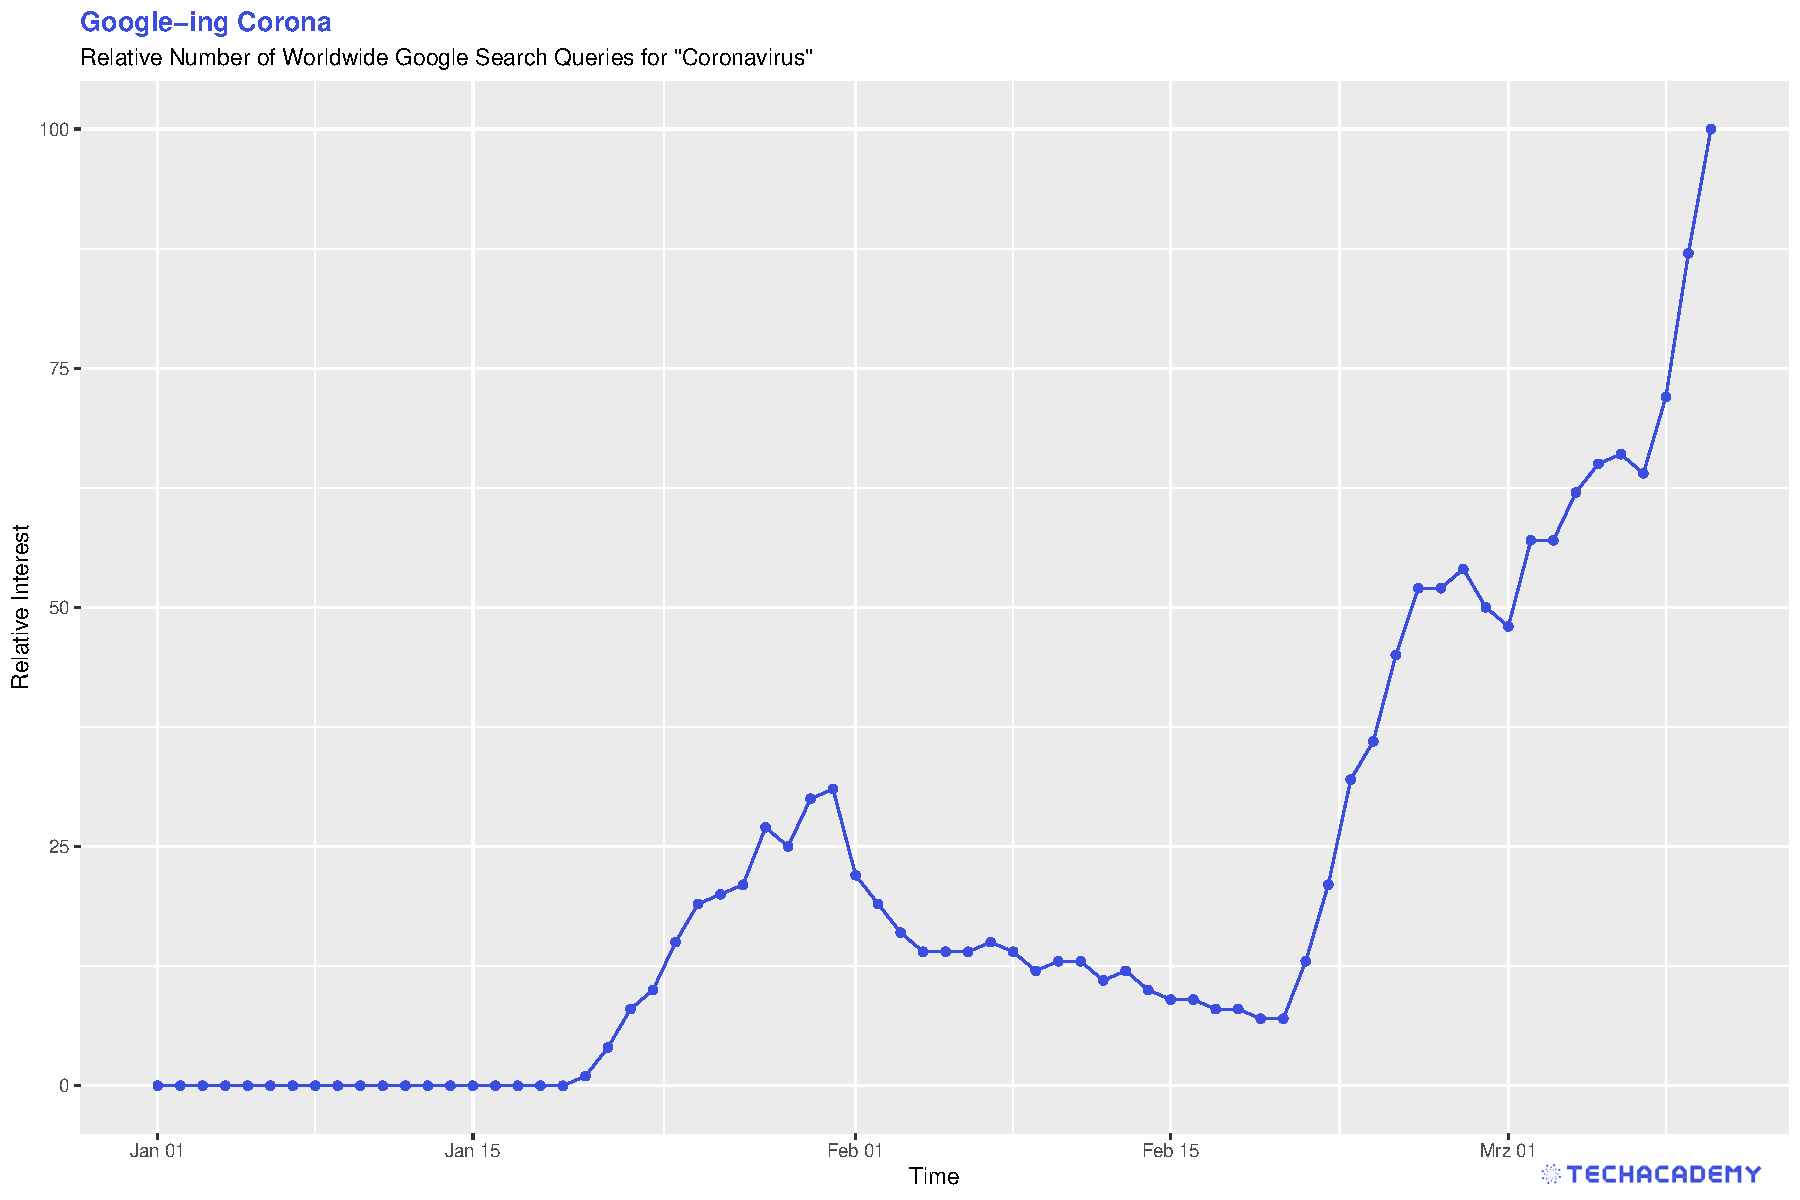
\includegraphics{output_files/figure-latex/unnamed-chunk-1-1.pdf}

\begin{verbatim}
> 'data.frame': 340 obs. of  8 variables:
>  $ symbol  : Factor w/ 7 levels "^GDAXI","^GSPC",..: 2 2 2 2 2 2 2 2 2 2 ...
>  $ date    : Factor w/ 50 levels "2020-01-02","2020-01-03",..: 1 2 3 4 5 6 7 8 9 10 ...
>  $ open    : num  3245 3226 3218 3242 3239 ...
>  $ high    : num  3258 3246 3247 3245 3267 ...
>  $ low     : num  3236 3222 3215 3232 3237 ...
>  $ close   : num  3258 3235 3246 3237 3253 ...
>  $ volume  : num  3.46e+09 3.46e+09 3.67e+09 3.42e+09 3.72e+09 ...
>  $ adjusted: num  3258 3235 3246 3237 3253 ...
\end{verbatim}

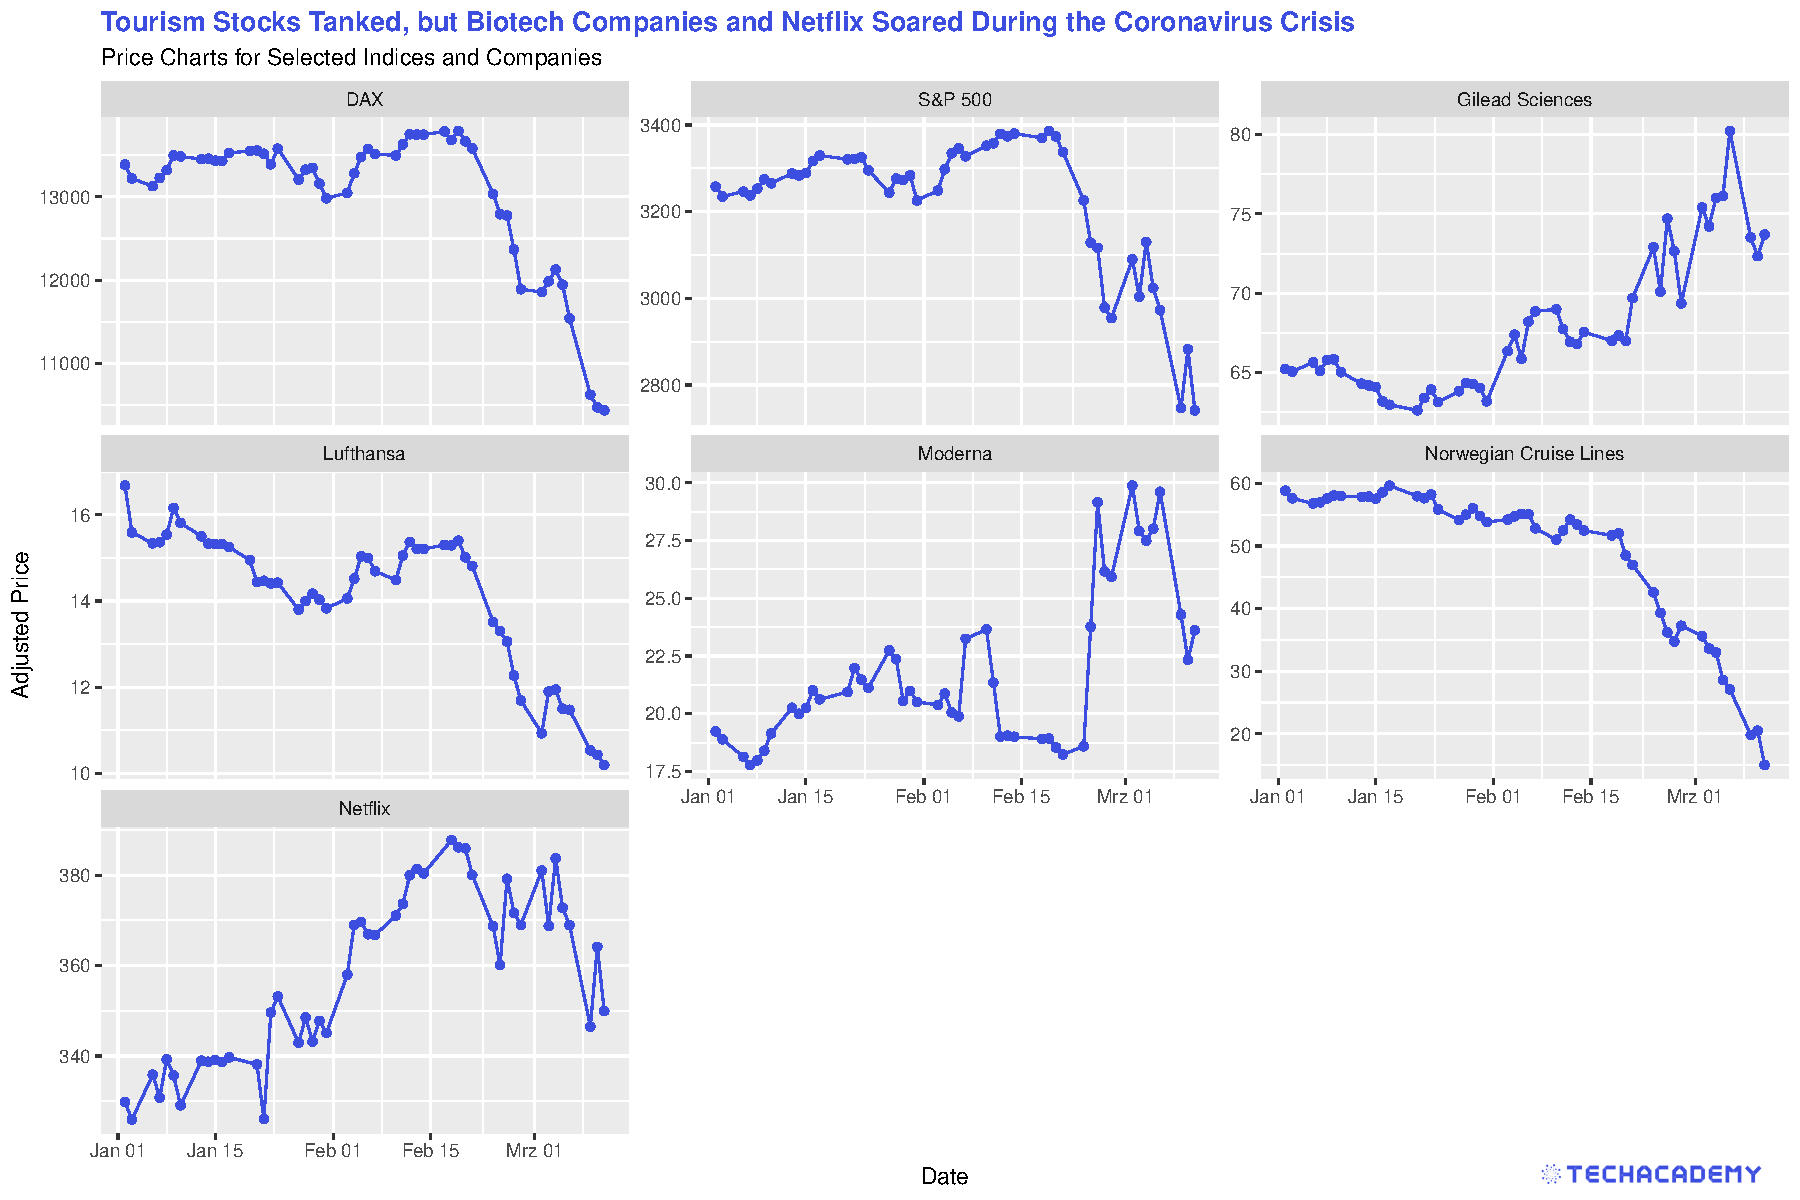
\includegraphics{output_files/figure-latex/unnamed-chunk-1-2.pdf}

\begin{verbatim}
> 'data.frame': 20200 obs. of  7 variables:
>  $ id       : int  1 2 3 4 5 6 7 8 9 10 ...
>  $ province : Factor w/ 297 levels "Adams, IN","Alachua, FL",..: NA NA NA NA NA 20 179 275 216 NA ...
>  $ country  : Factor w/ 114 levels "Afghanistan",..: 106 57 97 75 66 23 7 7 7 21 ...
>  $ latitude : num  15 36 1.28 28.17 2.5 ...
>  $ longitude: num  101 138 103.8 84.2 112.5 ...
>  $ time     : Factor w/ 50 levels "2020-01-22","2020-01-23",..: 1 1 1 1 1 1 1 1 1 1 ...
>  $ confirmed: int  2 2 NA NA NA NA NA NA NA NA ...
\end{verbatim}

\begin{verbatim}
> [1] 0
\end{verbatim}

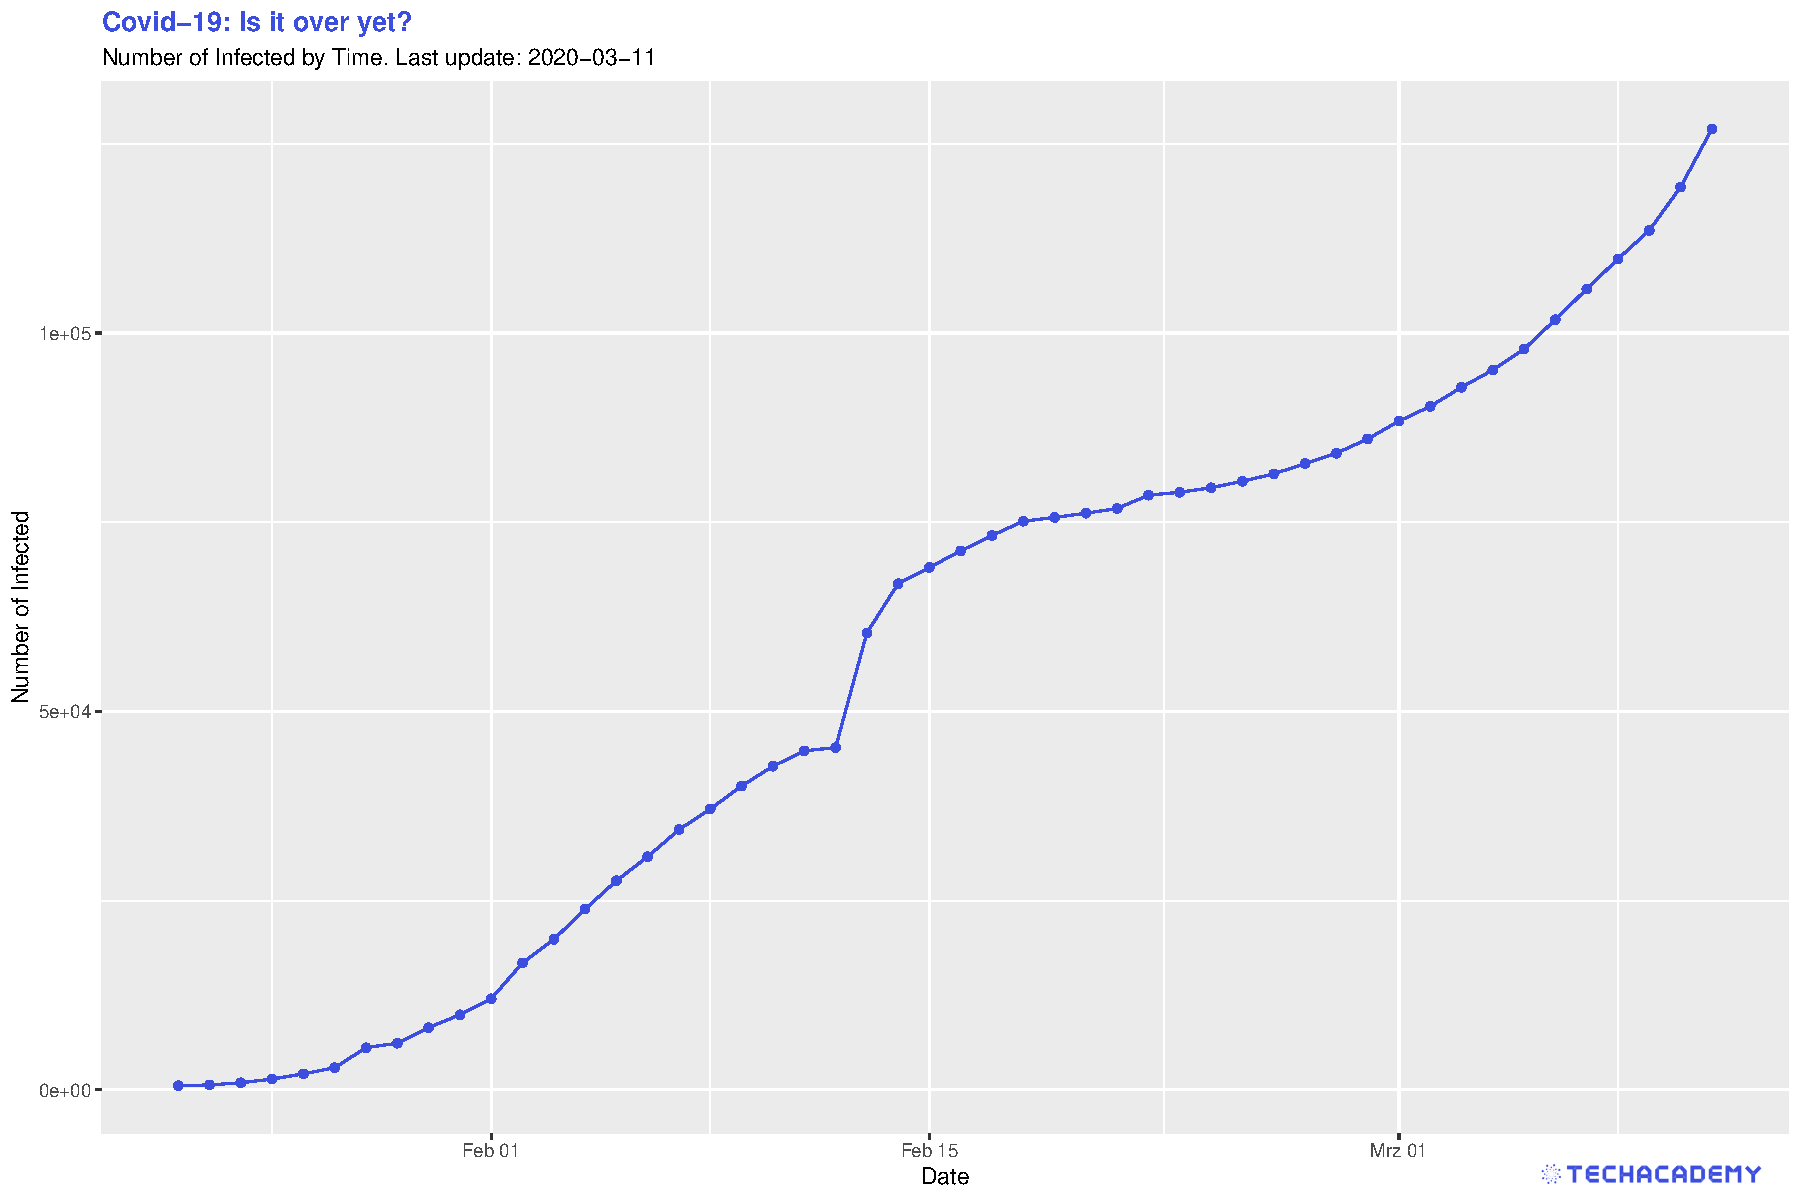
\includegraphics{output_files/figure-latex/unnamed-chunk-1-3.pdf} 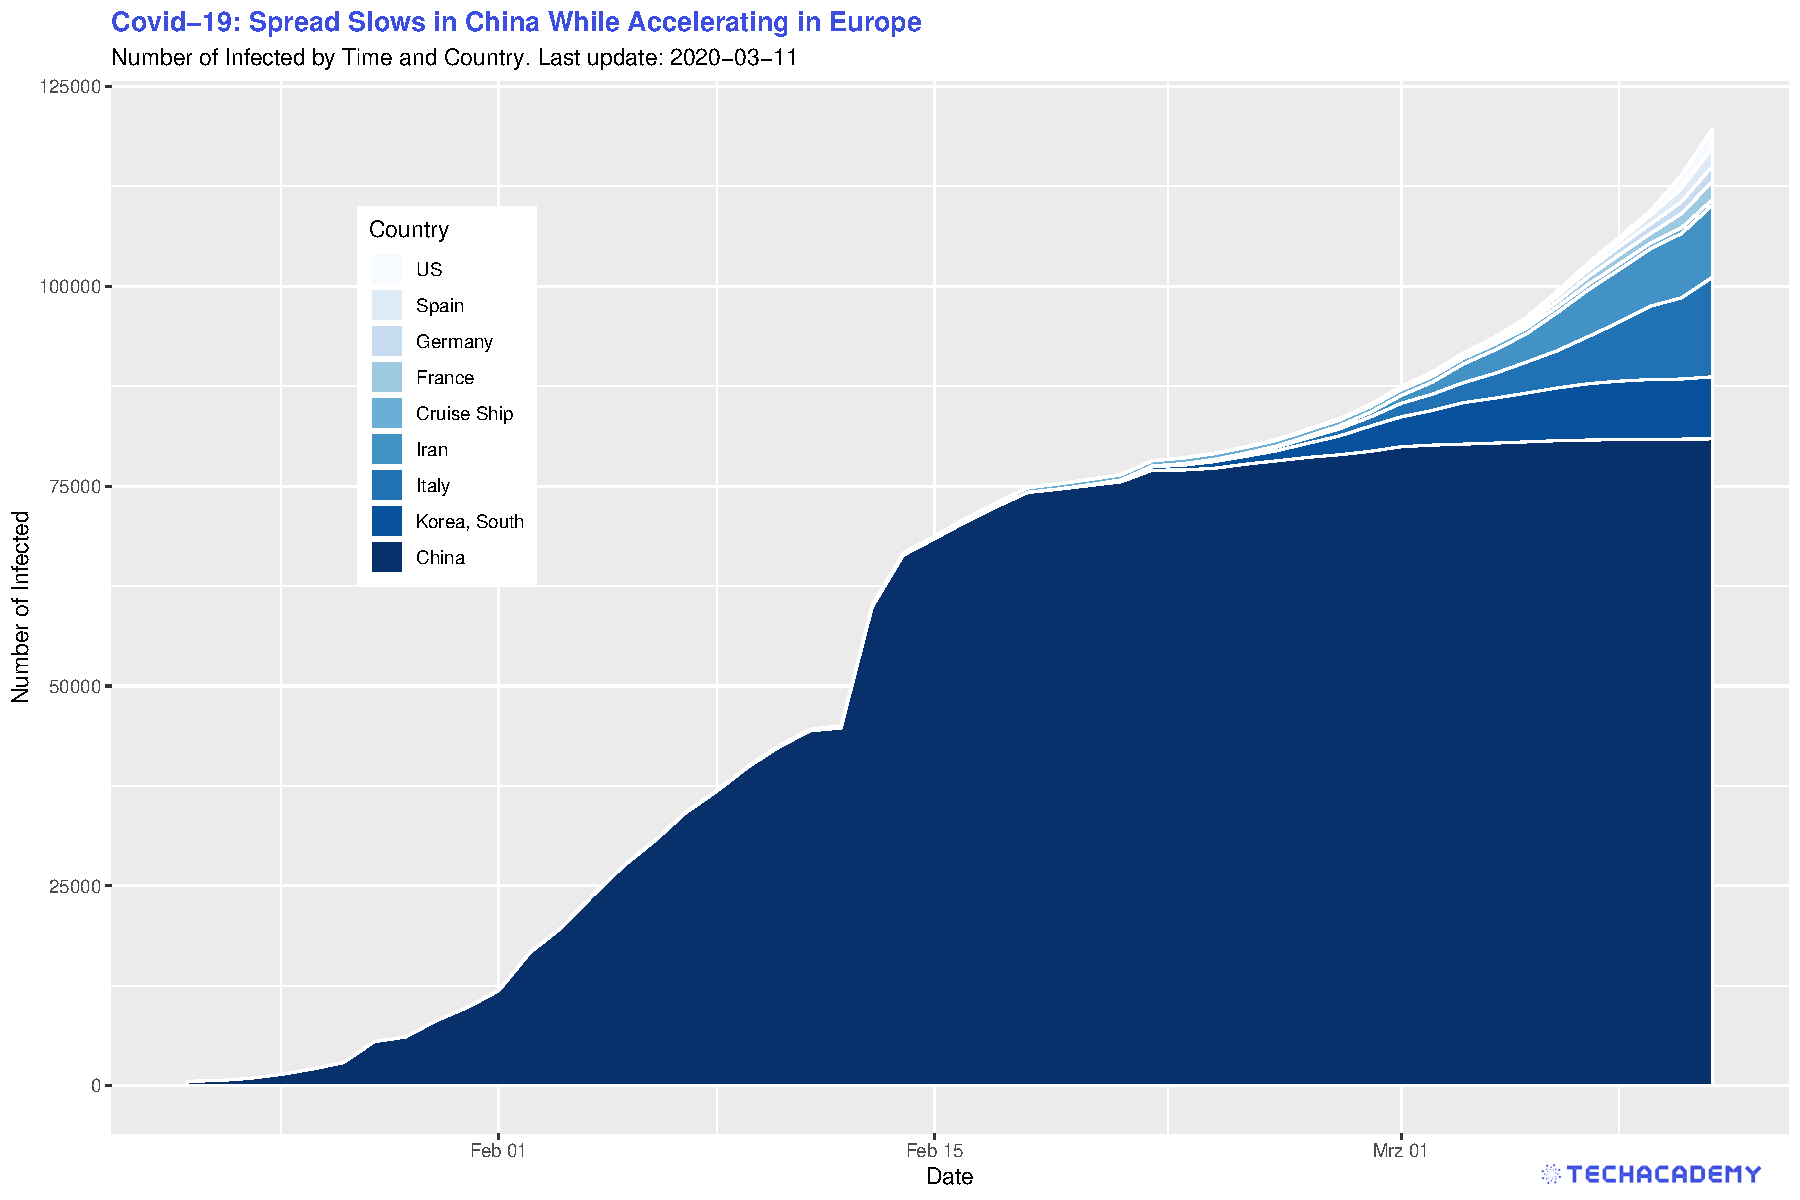
\includegraphics{output_files/figure-latex/unnamed-chunk-1-4.pdf} 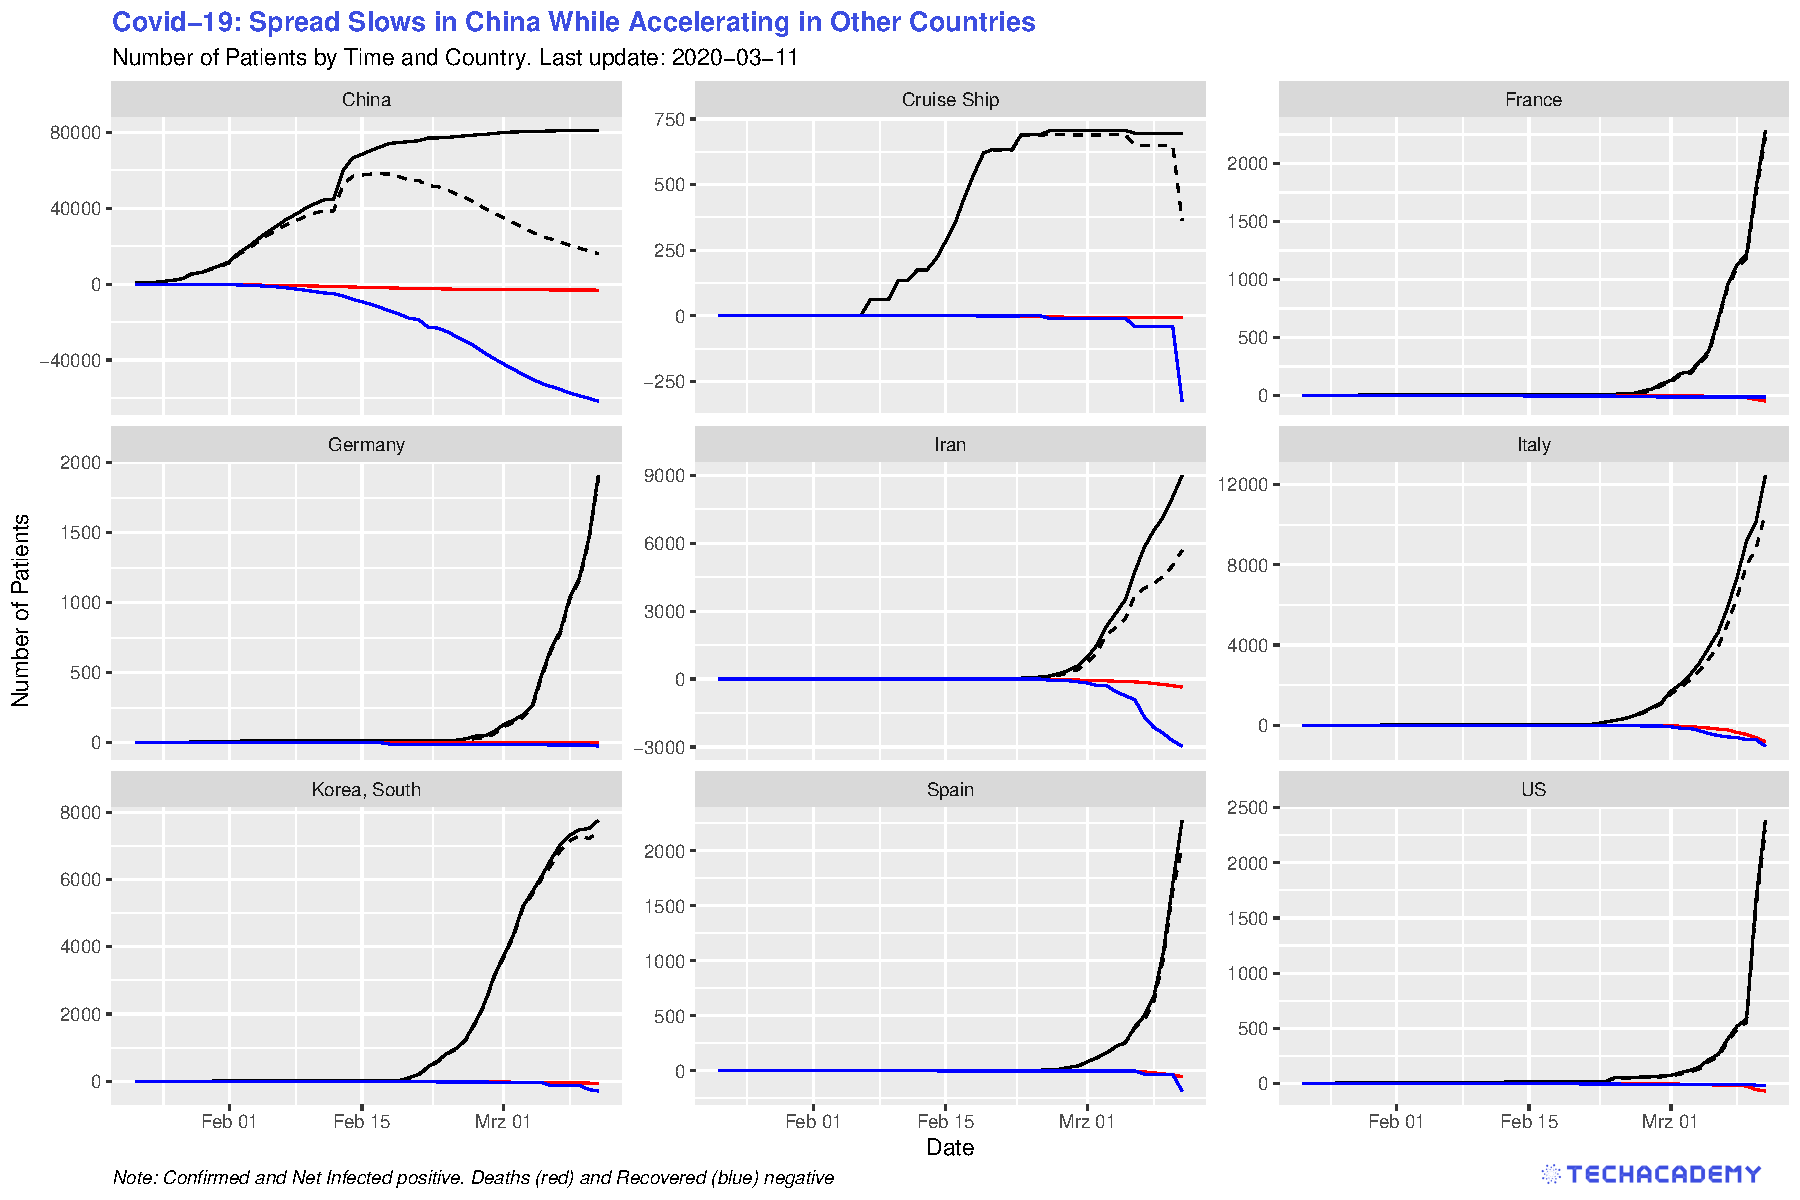
\includegraphics{output_files/figure-latex/unnamed-chunk-1-5.pdf} 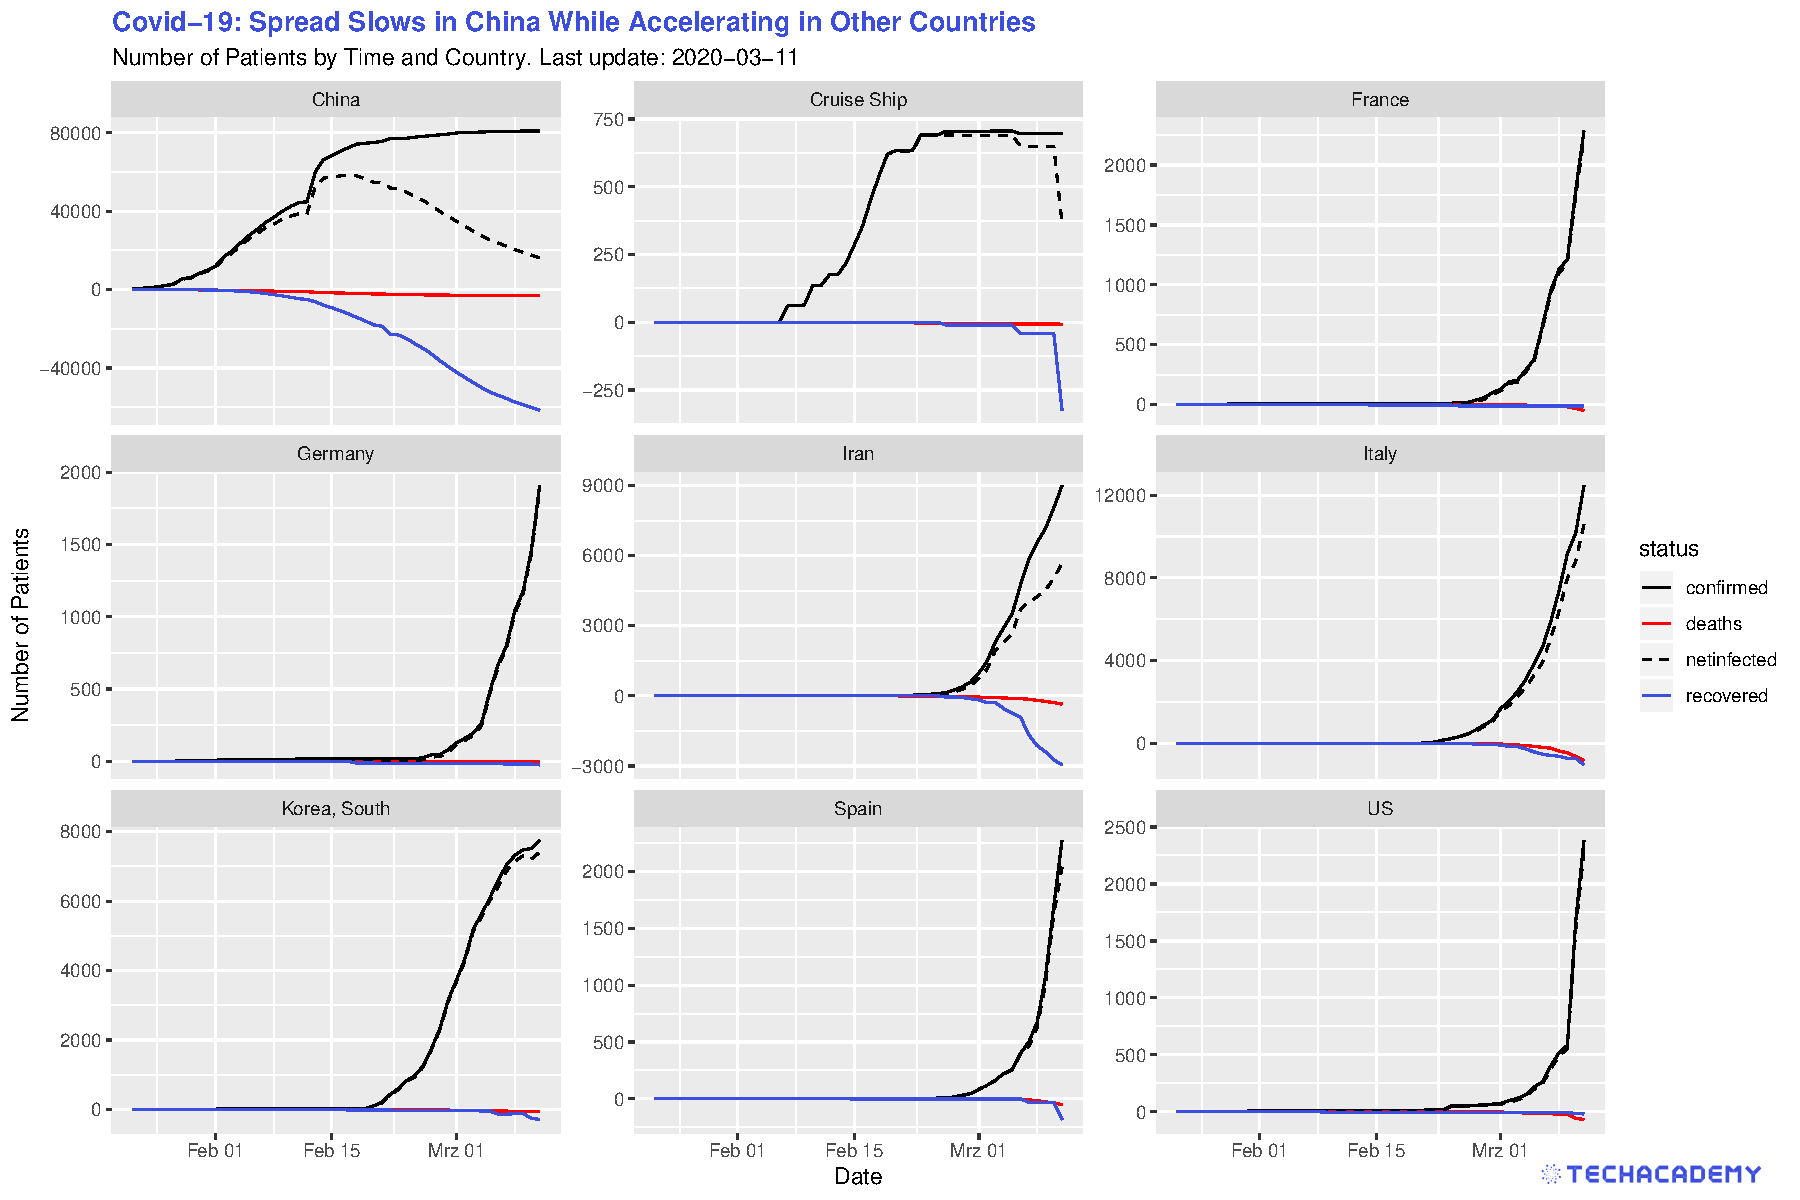
\includegraphics{output_files/figure-latex/unnamed-chunk-1-6.pdf} 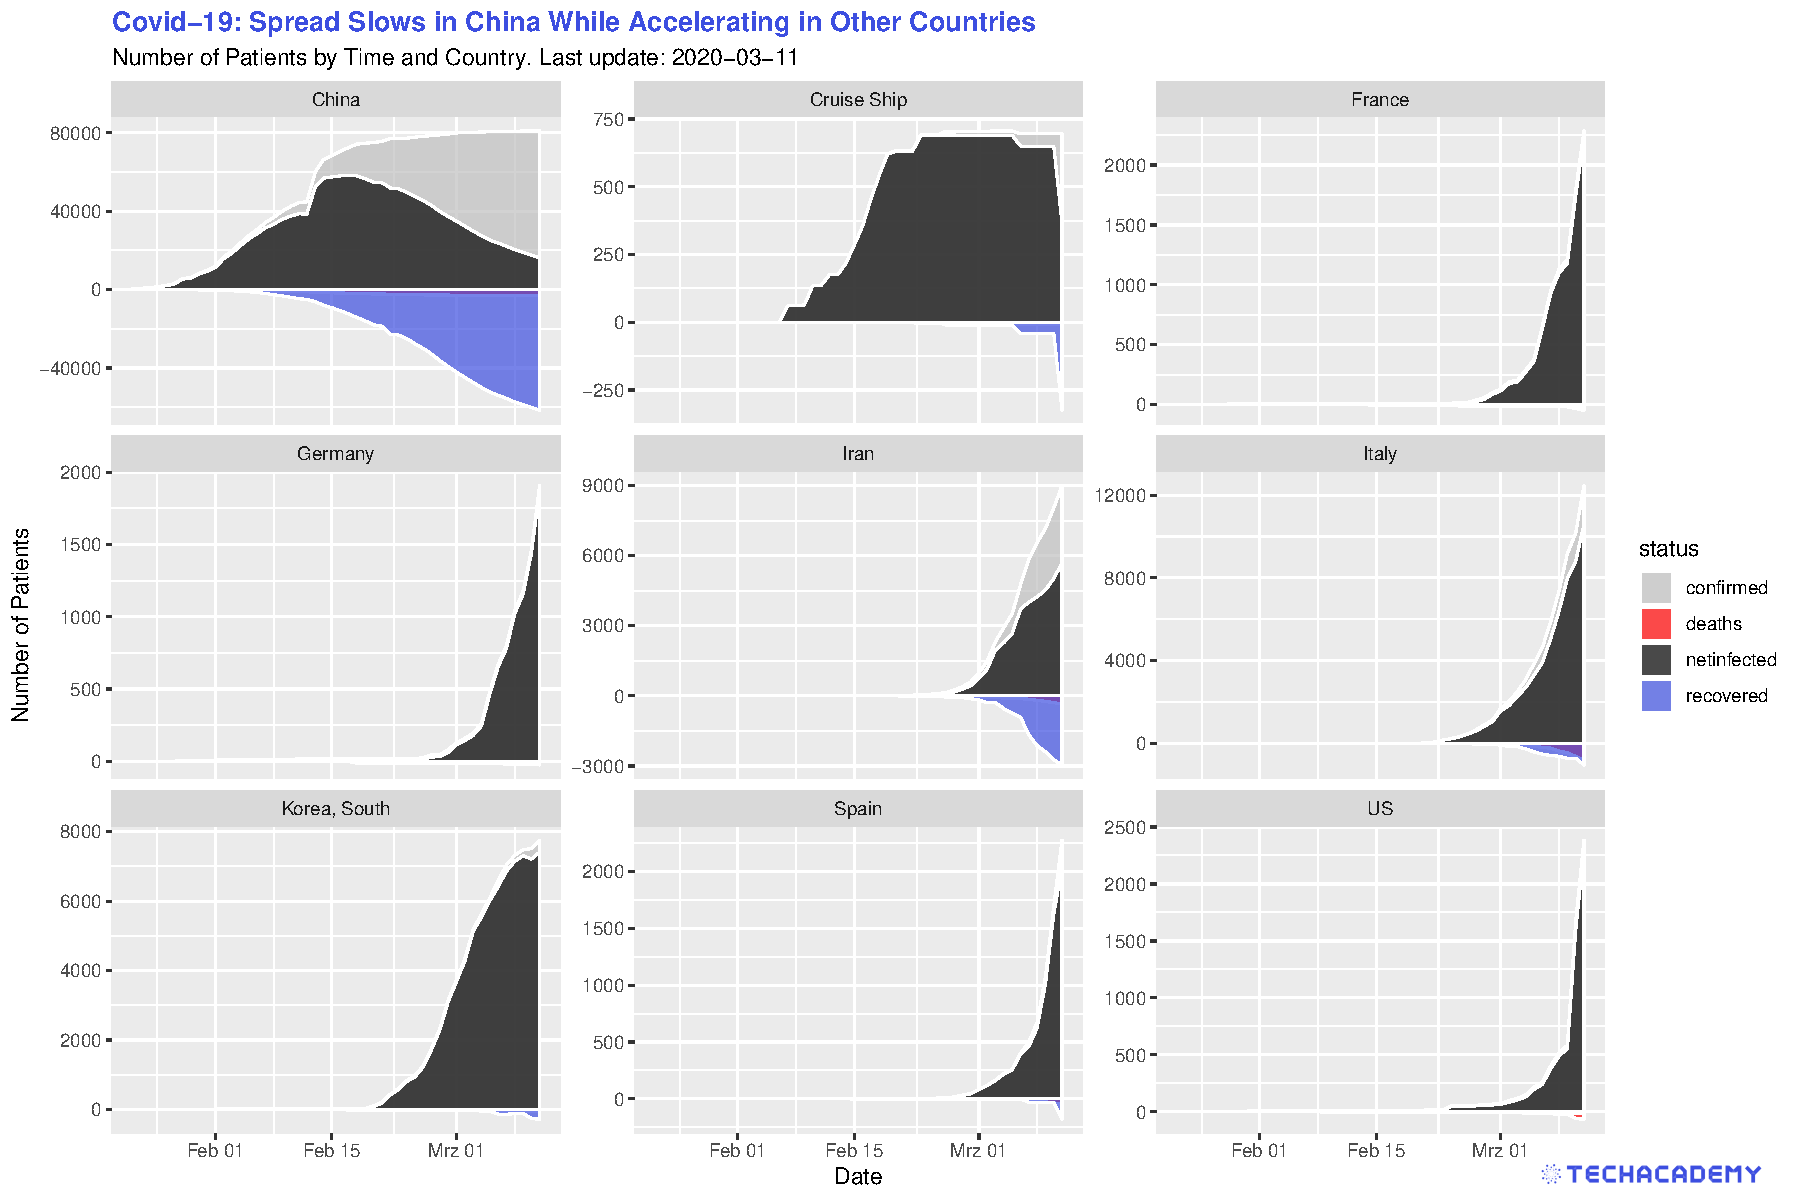
\includegraphics{output_files/figure-latex/unnamed-chunk-1-7.pdf} 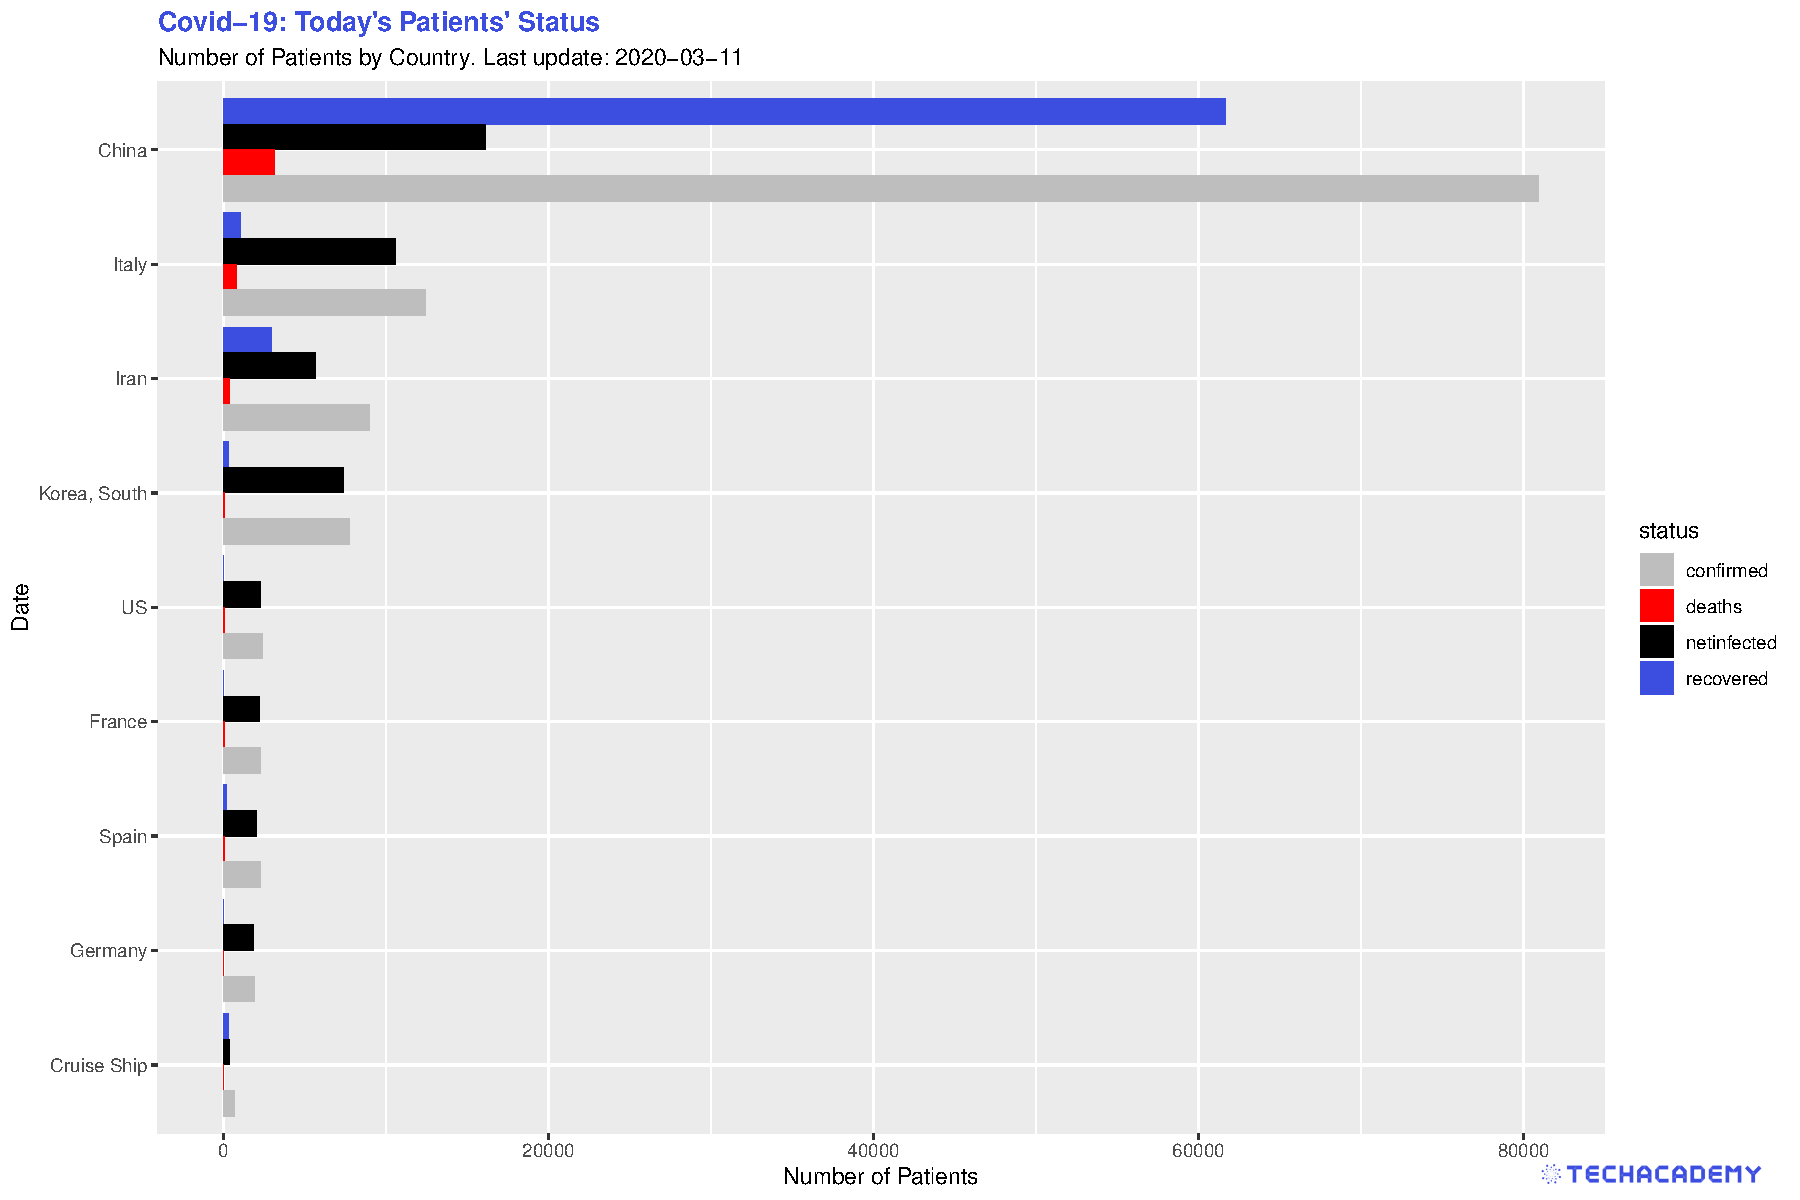
\includegraphics{output_files/figure-latex/unnamed-chunk-1-8.pdf} 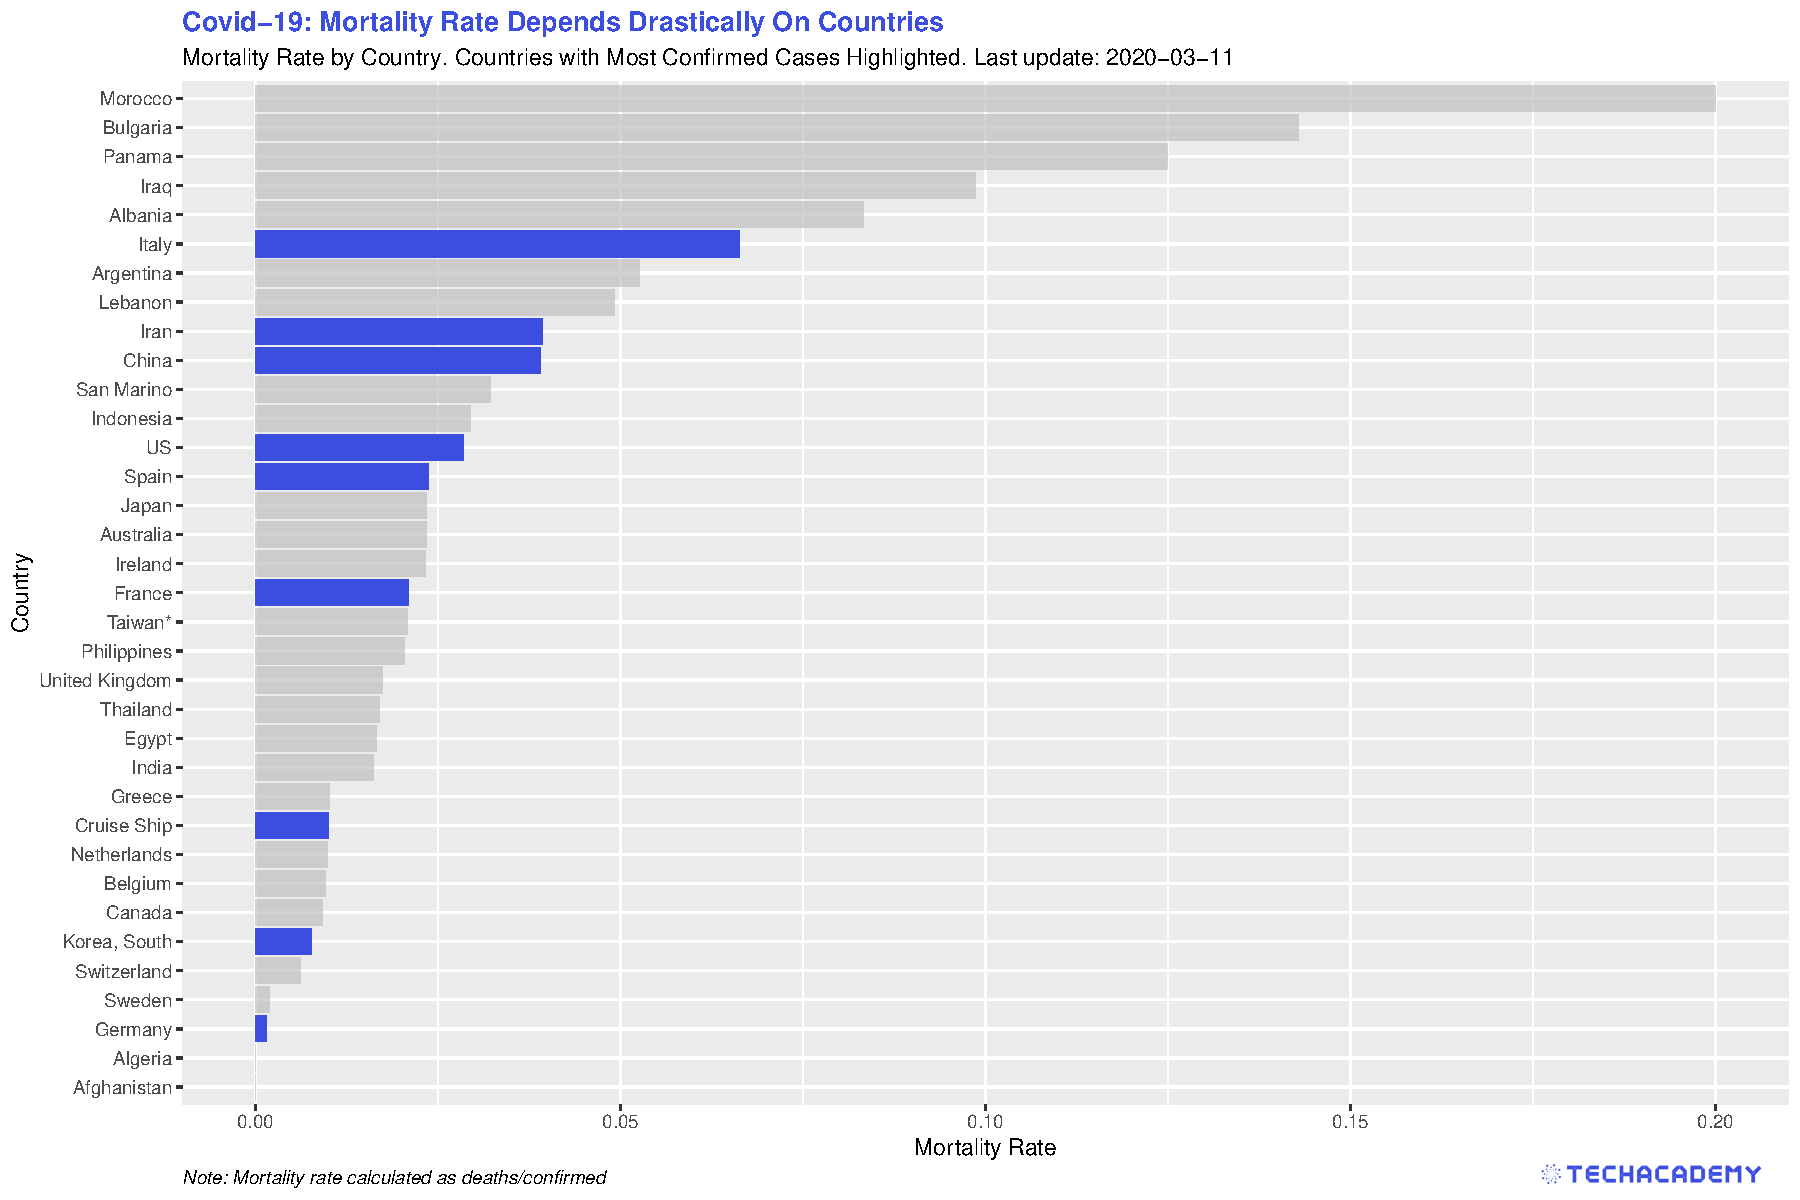
\includegraphics{output_files/figure-latex/unnamed-chunk-1-9.pdf} 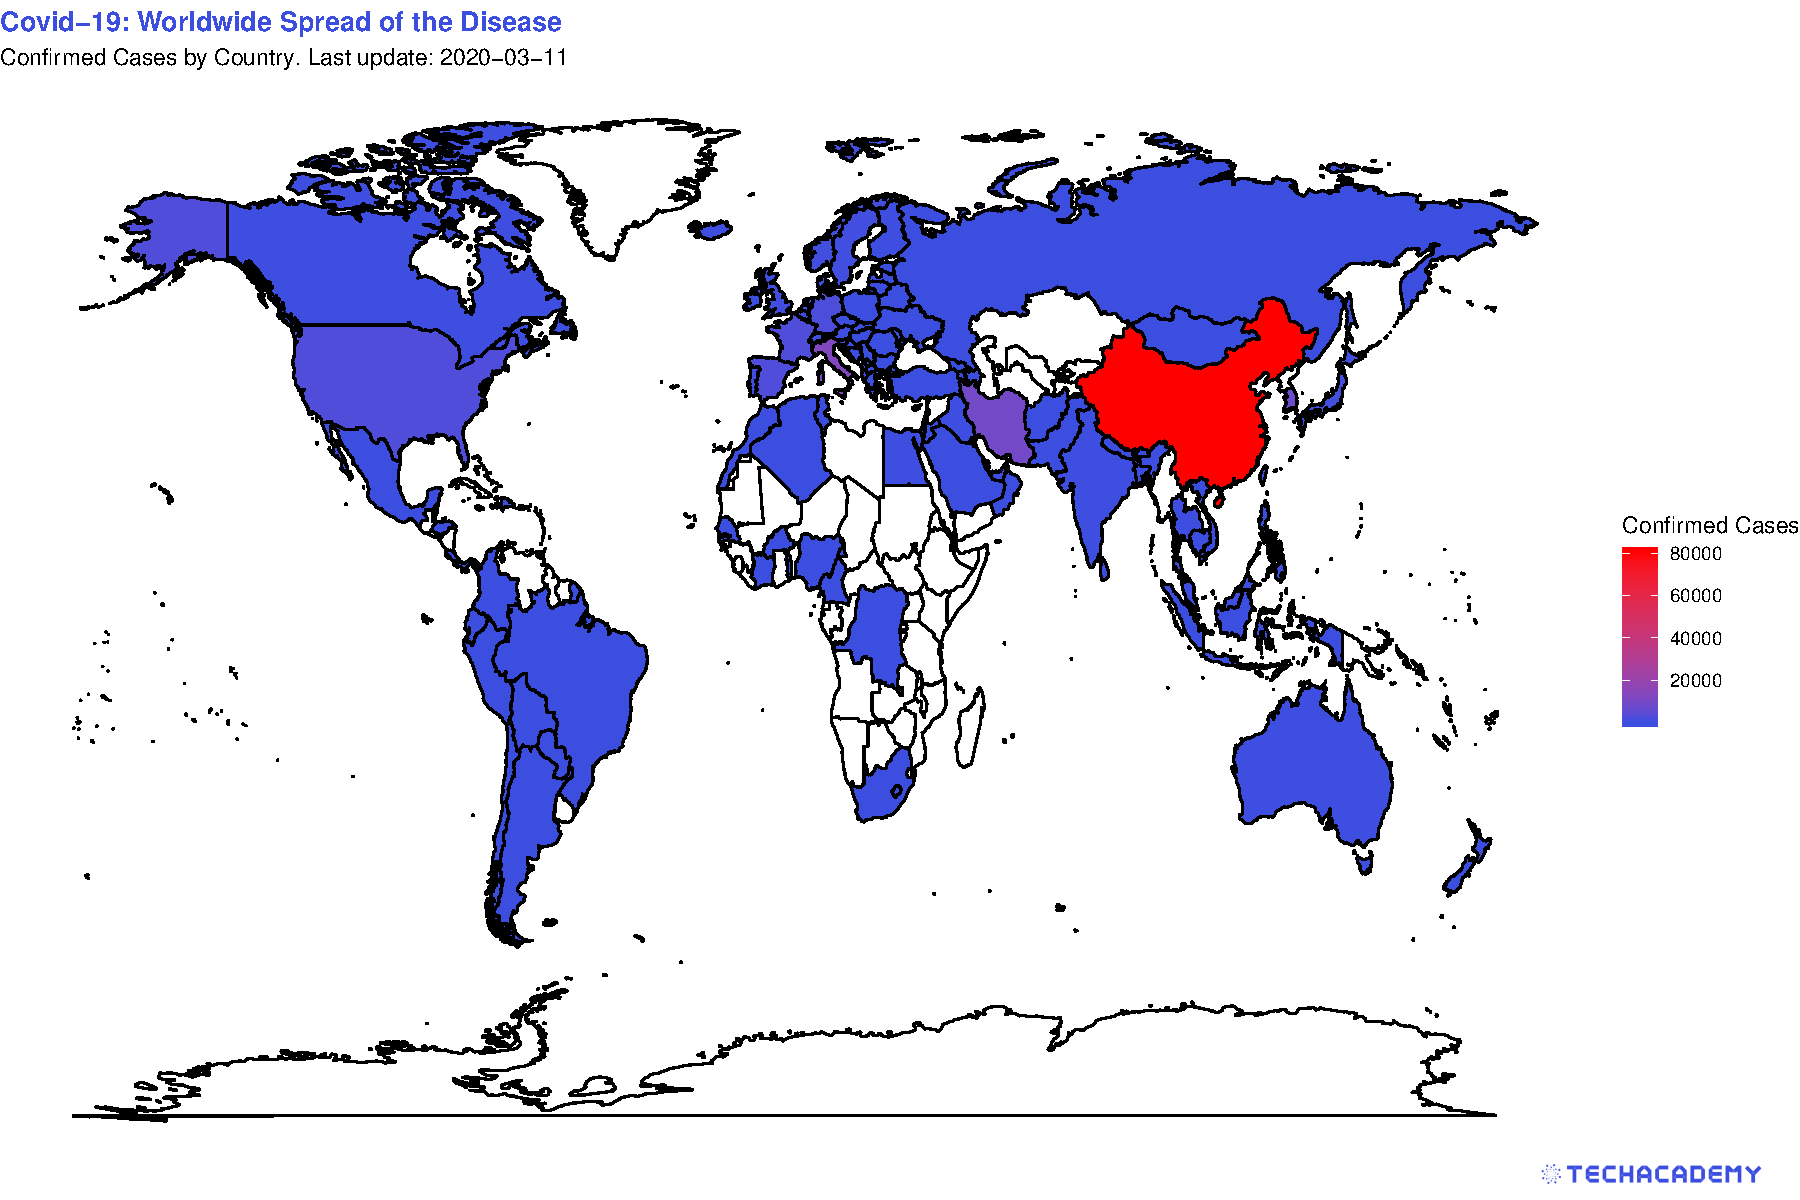
\includegraphics{output_files/figure-latex/unnamed-chunk-1-10.pdf} 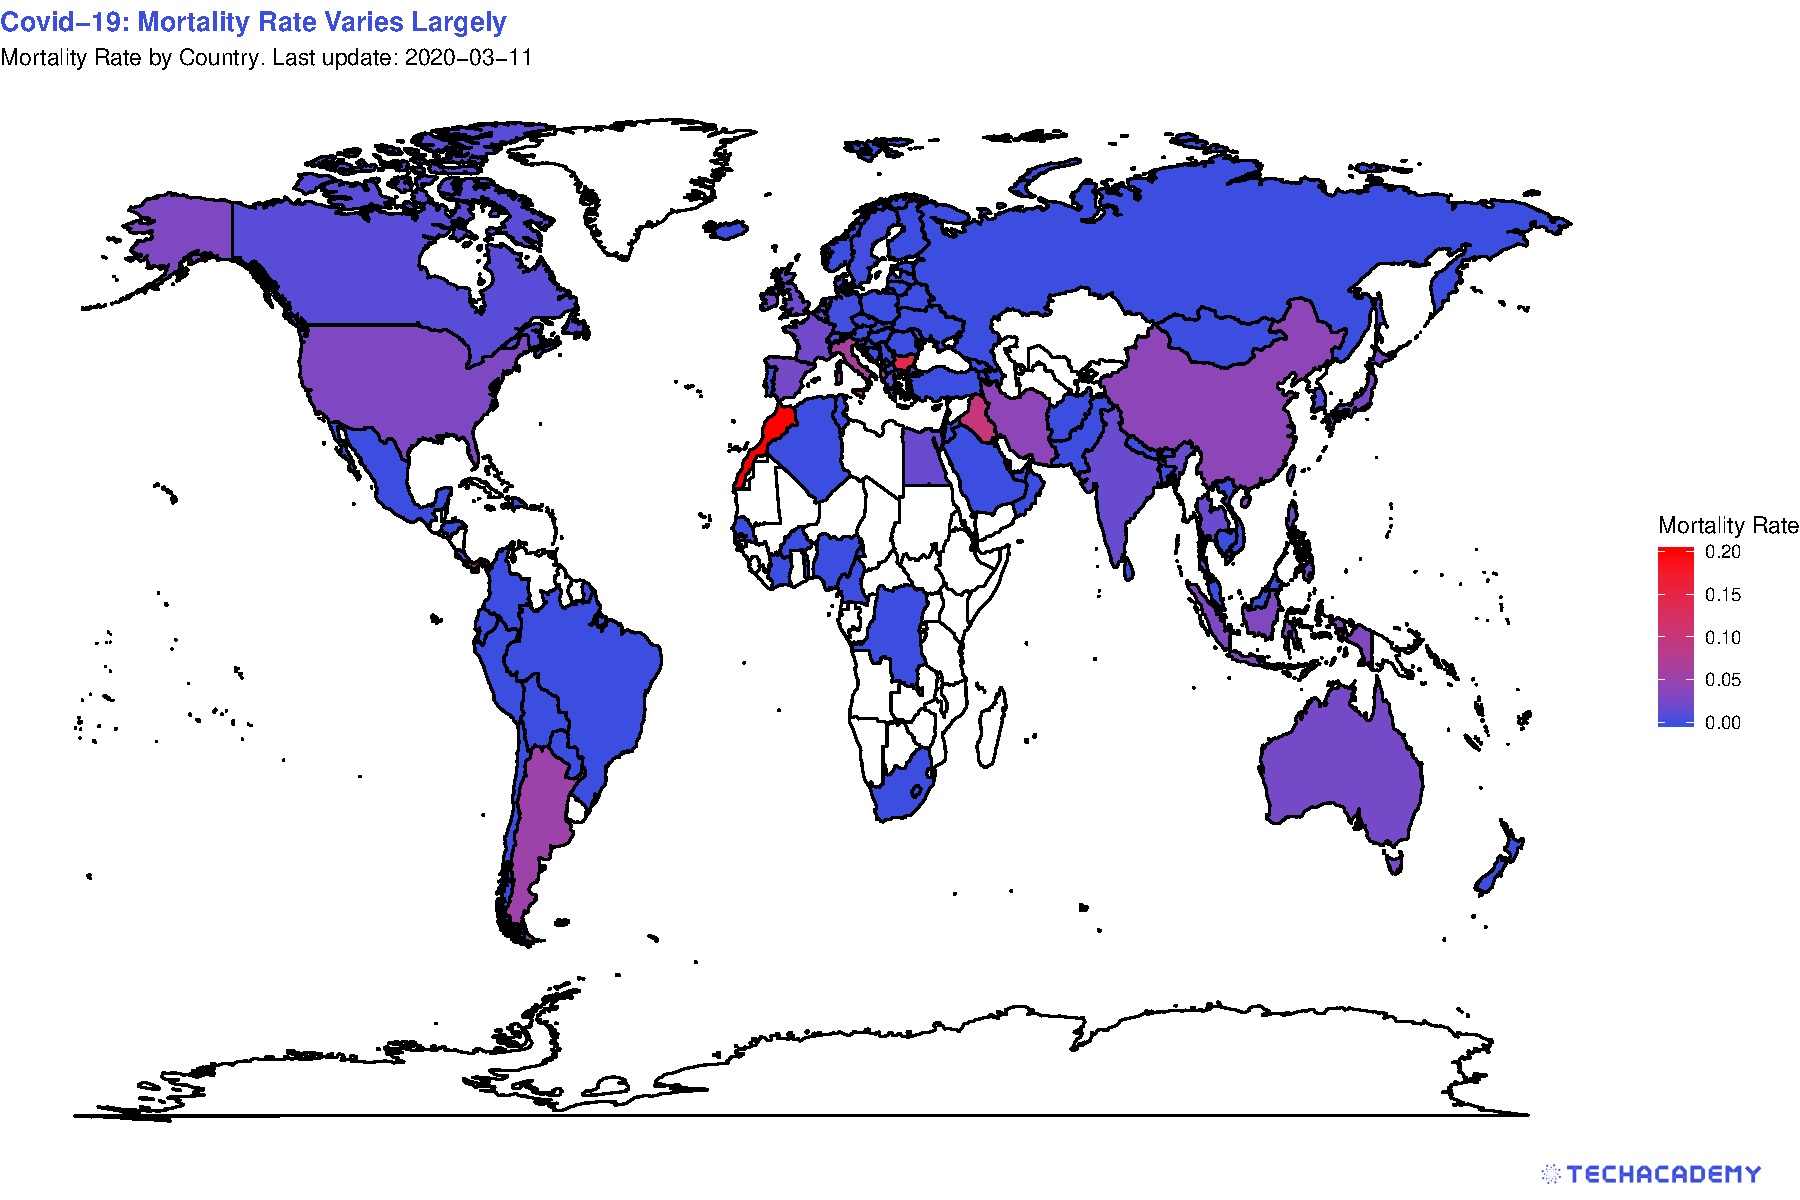
\includegraphics{output_files/figure-latex/unnamed-chunk-1-11.pdf} 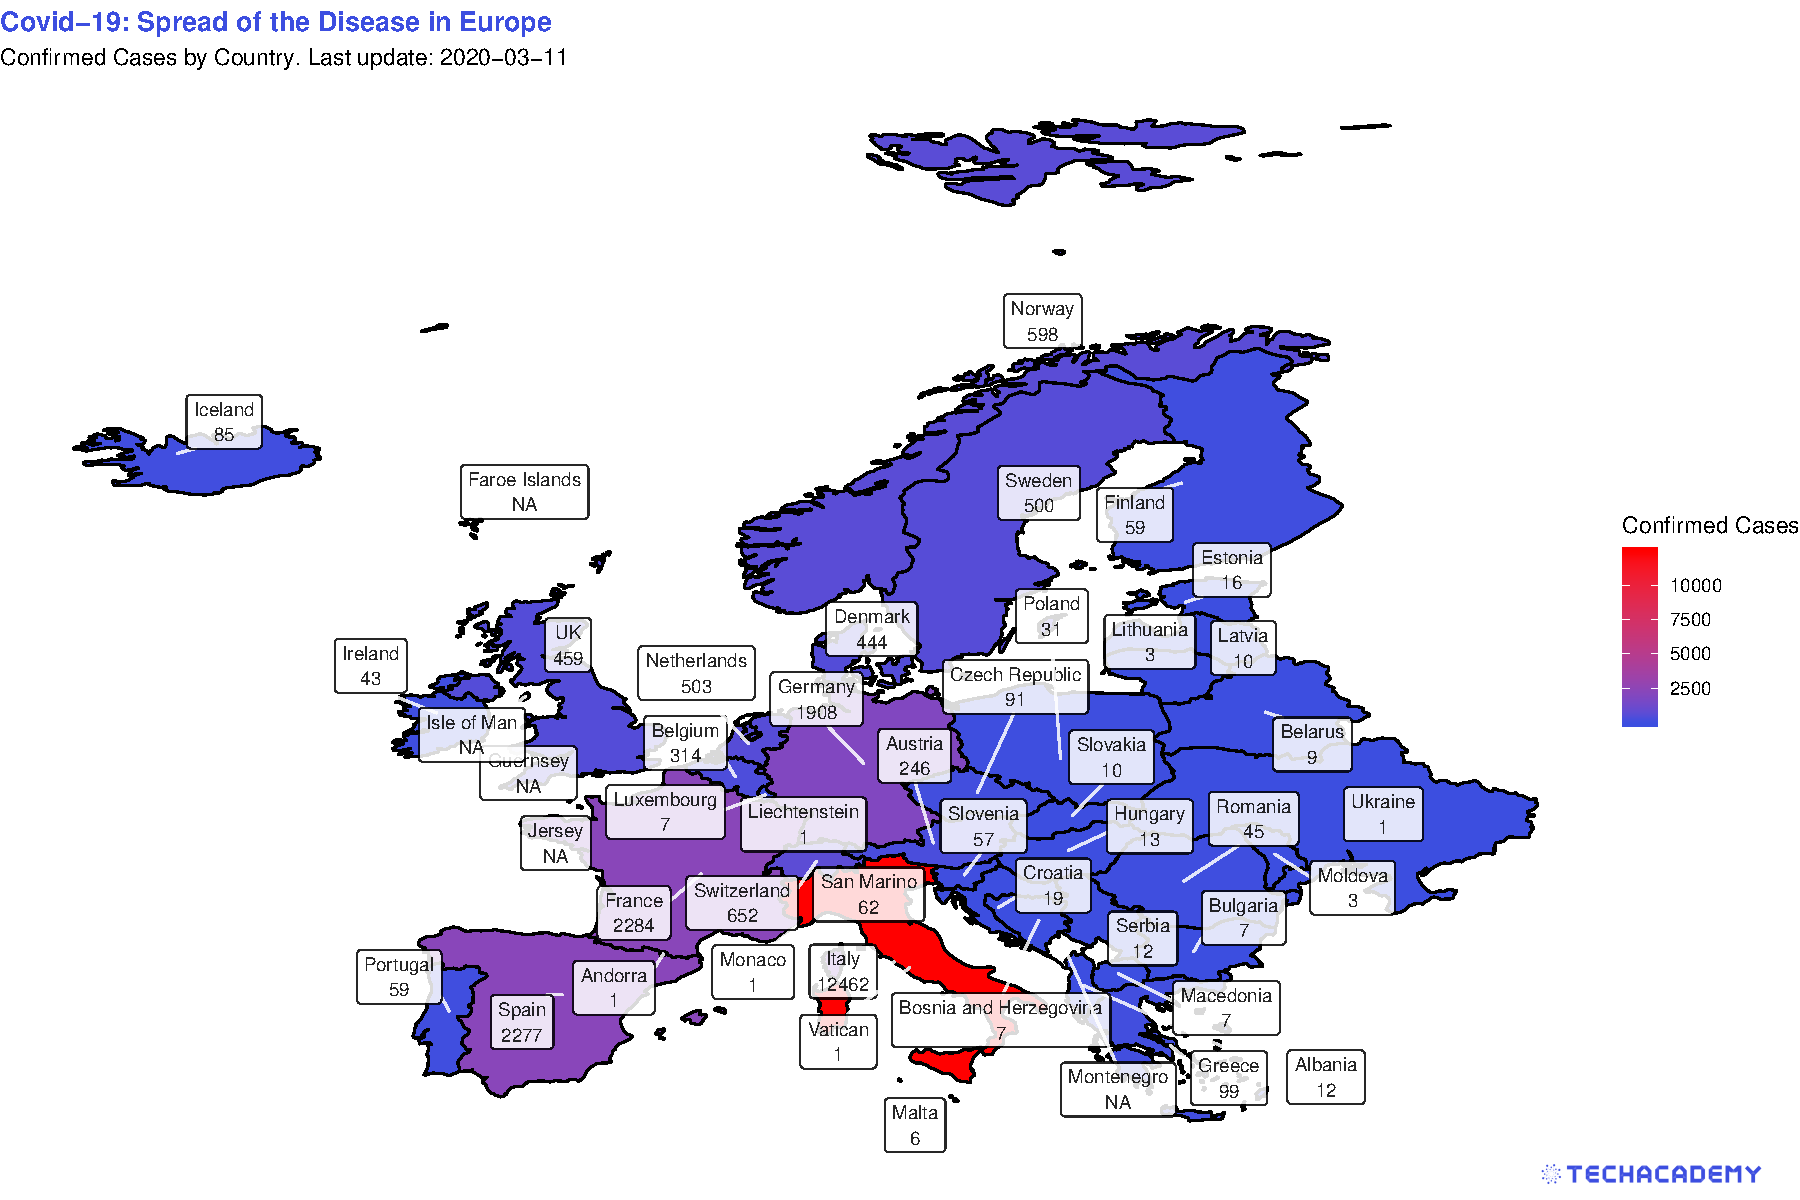
\includegraphics{output_files/figure-latex/unnamed-chunk-1-12.pdf}

\hypertarget{explorative-datenanalyse-lerne-den-datensatz-kennen-1}{%
\chapter{Explorative Datenanalyse -- Lerne den Datensatz kennen}\label{explorative-datenanalyse-lerne-den-datensatz-kennen-1}}

Wir haben in deinem Workspace bei \href{rstudio.cloud}{RStudio.cloud} bereits ein sogenanntes Assignment (Template Airbnb) hochgeladen.
Wenn du jetzt ein neues Projekt innerhalb des Workspaces ``Class of '19/20 \textbar{} TechAcademy \textbar{} Data Science with R'' erstellst, öffnet sich dein eigener Workspace, in dem wir schon ein paar Vorbereitungen für die erfolgreiche Bearbeitung getroffen haben.
So sind einerseits schon die benötigten Datensätze in deinem Working Directory abgelegt. Außerdem haben wir eine RMarkdown Datei erstellt, in der du strukturiert deine Aufgaben coden und letztendlich berichten kannst. Öffne also als ersten Schritt die Datei \texttt{Markdown\_Airbnb.Rmd}.

\hypertarget{datenimport--bereinigung--transformation-und-lineplot-calendar}{%
\section{Datenimport, -bereinigung, -transformation und Lineplot (Calendar)}\label{datenimport--bereinigung--transformation-und-lineplot-calendar}}

In diesem Abschnitt wendest du die grundlegensten Operationen an: Importieren, Bereinigen, Transformieren und am Schluss eine erste einfache Visualisierung des Datensatzes.
Zuerst muss der Datensatz aus deiner Ordnerstruktur in den Workspace geladen werden.
Importiere den \texttt{calendar} Datensatz in deinen Workspace und benenne das Objekt danach.

Verschaffe dir nun einen Überblick über den Datensatz.
Wie ist dieser aufgebaut und welche Variablen sind darin enthalten?
Was fällt dir dabei auf?
Dafür kannst du zum Beispiel folgende Funktionen nutzen:

Bevor du dir überlegst, welche statistischen Methoden für die Vorhersage geeignet sein könnten, ist es immer nützlich sich die Zusammenhänge zwischen den Variablen visuell darzustellen.
Wie bereits oben angesprochen nennt man diesen Prozess Exploratory Data Analysis (EDA).

Bevor wir damit starten können, müssen wir den Datensatz zuerst ein wenig bearbeiten, damit die Funktionen diesen verarbeiten können.
Das klingt einfacher als gedacht --- sehr oft sind die Daten in einem unbrauchbaren Format.
In unserem Fall ist zum Beispiel die Preis-Variable \texttt{price} als string-Variable gespeichert.
Damit R diese verarbeiten kann, müssen wir ein Zeichen aus den Beobachtungen entfernen und die Variable in ein \texttt{numeric} Format bringen.
Dafür kannst du die Funktionen \texttt{str\_remove\_all()} oder \texttt{gsub()} in Kombination mit \texttt{as.numeric()} verwenden.

Damit der nächste Schritt leichter fällt, müssen wir noch die logische Variable \texttt{available} von einem \texttt{factor} zu einem \texttt{boolean} Datentyp konvertieren.
Nutze dafür die \texttt{ifelse()} Funktion und ersetze jeweils ``f'' und ``t'' mit den dazugehörigen logischen Werten \texttt{FALSE} bzw. \texttt{TRUE}.
Transformiere als letzten Schritt die Datumsvariable von in das R Datumsformat \texttt{date}.
Erinnerst du dich an die \texttt{as.numeric()} Funktion?
R besitzt eine ähnliche Funktion zur Konvertierung in Datums-Variablen.

Unser Ziel ist es nun, die Anzahl der verfügbaren Airbnb Apartments über das nächste Jahr in einem einfachen Lineplot darzustellen.
Jedoch ist unser Datensatz dafür noch nicht im richtigen Format -- aktuell hat jedes Apartment einen Eintrag für jeden der kommenden 365 Tage und jeweils eine Variable, die uns anzeigt, ob das Apartment an diesem Tag verfügbar ist.
Unser transformierter Datensatz soll jedoch diese Infomationen zusammenfassen und nur einen einzigen Eintrag für jeden Tag im nächsten Jahr sowie die aggregierte Anzahl an verfügbaren Airbnbs in Berlin enthalten.
Das R package \texttt{dplyr} ist die erste Wahl für diese Art von Transformations-Aufgaben.
Falls du davon noch nichts gehört hast, absolviere den DataCamp Kurs dazu und/oder zu Exploratory Data Analysis.
Nutze die \texttt{dplyr} Funktionen \texttt{group\_by()} und \texttt{summarise()} dafür und speichere den daraus resultierenden Datensatz in einem neuen data frame ab, den du z.B. \texttt{avail\_by\_date} nennen kannst.
Nutze für diese Aufgabe gerne das \texttt{dplyr} Cheat Sheet, auf welchem die Transformationen visuell dargestellt werden.

Jetzt haben wir den Datensatz in ein brauchbares Format gebracht und können die Ergebnisse visualisieren.
Bevor du dich an das Coden machst, überlege dir, was du von diesem Plot erwartest und wie er aussehen könnte.
Vergleiche diese Erwartungen dann mit dem tatsächlichen Plot und versuche die markanten Stellen mit deiner Intuition zu erklären.
Plotte dafür einen einfachen Lineplot, welcher die Anzahl der verfügbaren Apartments über die nächsten 365 Tage zeichnet.
Du kannst dafür das \texttt{base} Package mit der Funktion \texttt{plot()} oder gleich das umfangreiche und sehr flexibel einsetzbare Grafikpackage \texttt{ggplot2} verwenden.

Starte einfach und verfeinere dann deinen Plot.
So in etwa kann dein erstes Ergebnis ausschauen:

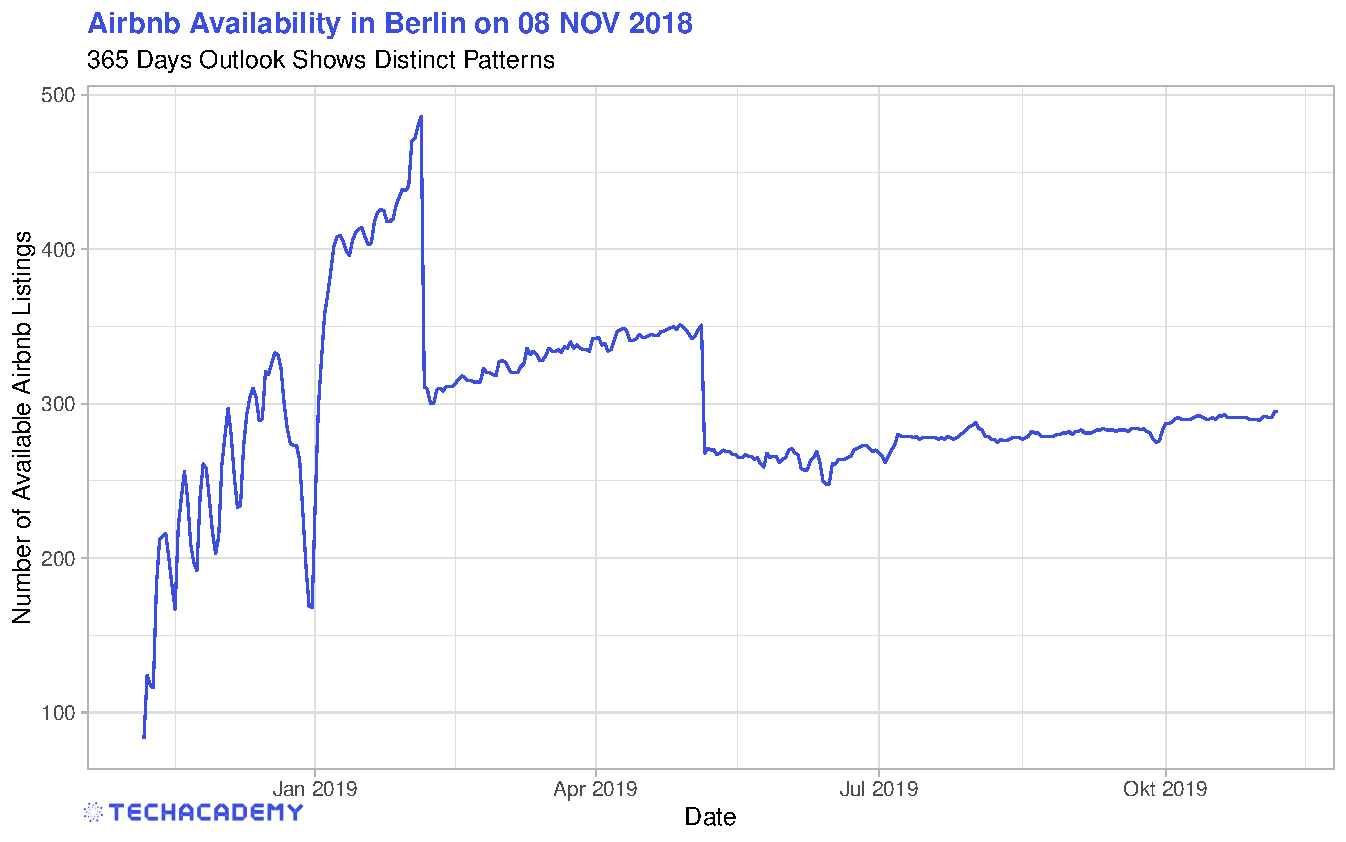
\includegraphics[width=1\linewidth,height=500   extheight]{plots/1_3_AvailabilityOutlook}

Überlege dir nun, was der Verlauf des Graphen bedeutet: Warum sind so viele regelmäßige Muster in der Verfügbarkeit?
Und warum gibt es immer wieder deutliche und abrupte Verringerungen der Verfügbarkeit?
Unten siehst du einen Beispielplot, wie man mit \texttt{ggplot2} einen einfachen Plot verfeinern kann und somit die Aufmerksamkeit der Betrachter auf bestimmte Muster lenken kann.
Halte dich jedoch nicht zu lange mit kleinen Feinheiten und Spielerein auf -- falls du am Schluss noch Zeit hast, kannst du dich noch einmal damit befassen.

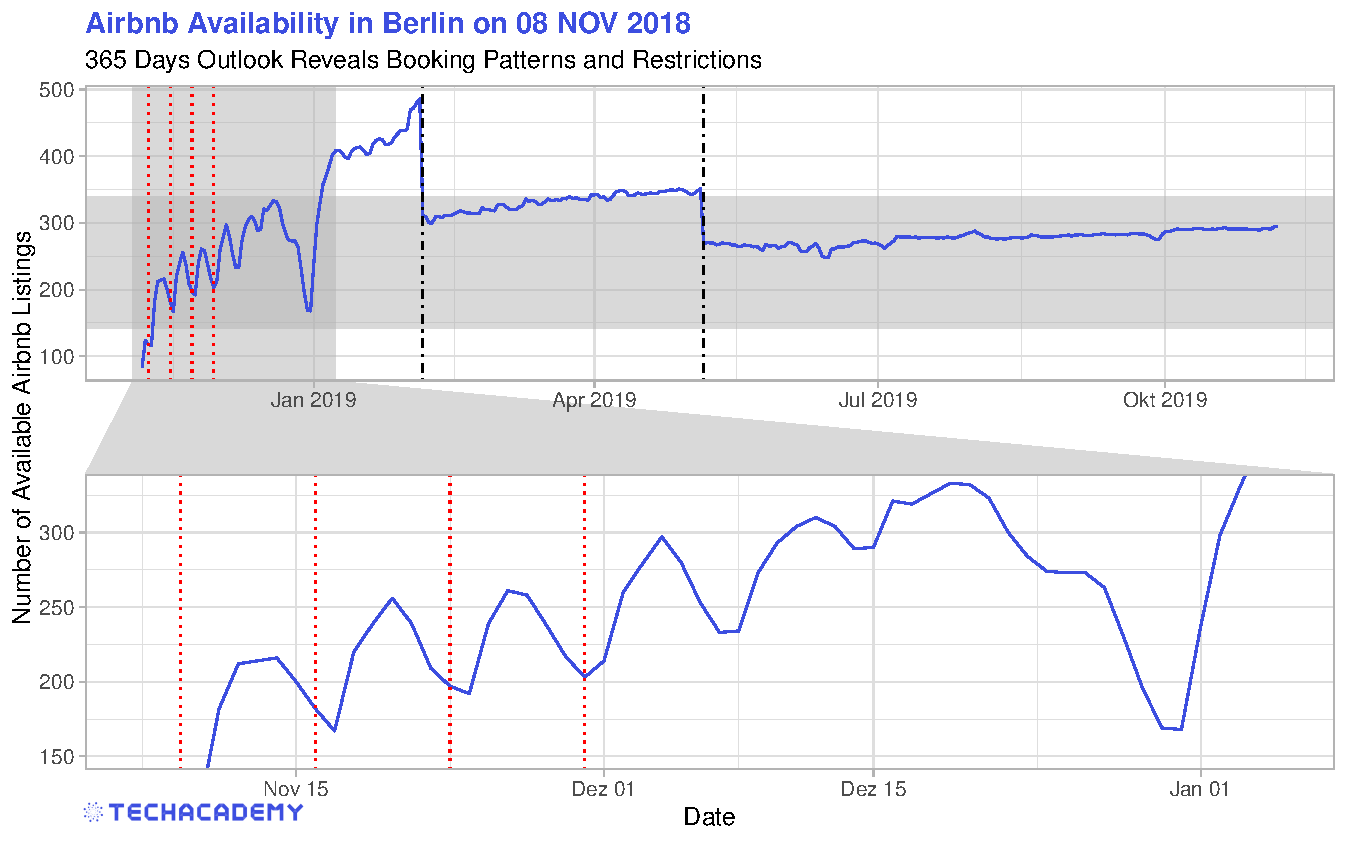
\includegraphics[width=1\linewidth]{plots/1_3_AvailabilityOutlook_advanced}

\hypertarget{visualisiere-individuelle-airbnb-angebote-listings}{%
\section{Visualisiere individuelle Airbnb-Angebote (listings)}\label{visualisiere-individuelle-airbnb-angebote-listings}}

Nachdem wir uns im ersten Schritt die Verfügbarkeit über die Zeit hinweg mithilfe des \texttt{calendar}-Datensatzes angeschaut haben, möchten wir nun etwas mehr über die Preisstrukturen der zur Verfügung stehenden Apartments herausfinden.
Dazu benötigen wir den \texttt{listings}-Datensatz, welchen wir wie gewohnt in den Workspace laden können.
Beim genaueren Betrachten fällt auf, dass die Spalte \texttt{price} und \texttt{cleaning\_fee} ein \$-Zeichen enthalten.
Dies ist für uns zwar wichtig, damit wir wissen, um welche Währungen es sich handelt.
Jedoch kann R damit nichts anfangen und weiß nicht, wie der String in eine Zahl umgewandelt werden soll.

Daher muss analog zur ersten Aufgabe für diese Spalten das Dollarzeichen gelöscht werden.
Hinzu kommt, dass in manchen Spalten ein Komma als Tausender-Trennzeichen verwendet wird.
Diese Kommas in der \texttt{price}-Spalte können auf die gleiche Weise entfernt werden.
Da du die gleiche Vorgehensweise für die Spalten \texttt{price} und \texttt{cleaning\_fee} benutzt, bietet sich hier ein \texttt{for}-loop an.
Implementiere diese Schleife in einer selbst geschriebenen Funktion \texttt{clean\_price()}, damit du dir besonders beim Vorhersageteil viele Zeilen Code sparst.

Da wir jetzt den Datensatz gesäubert haben, können wir uns die Preisstruktur der verschiedenen Stadtteile genauer anschauen.
Zunächst möchten wir wissen, wie hoch der Durchschnittspreis und die zugehörige Standardabweichung für jeden Stadteil ist.
Erstelle dazu eine Liste mit den Namen der verschiedenen Stadtteile und dem \texttt{mean} sowie der \texttt{sd}.
Verwende dafür zum Beispiel wieder die \texttt{dplyr}-Funktionen \texttt{group\_by()} und \texttt{summarise()}.

Nun möchten wir die Verteilung der Preise im durchschnittlich teuersten und im günstigsten Stadteil gegenüber stellen.
Überlege dir dafür, welche Art von Diagramm du im Kurs kennengelernt hast und hier am meisten Sinn ergibt.
Hast du das Diagramm erstellt, musst du vermutlich einen Teil der Ausreißer mit extrem hohen Preisen herausfiltern, um einen aussagekräftigen Plot zu erhalten. Das Filtern kannst du aber ganz einfach in den Plot-Spezifikationen mit \texttt{xlim} bzw. \texttt{ylim} durchführen.

Bei Airbnb können die verfügbaren Apartments nach Preis sortiert werden und dem Kunden in der entsprechenden Reihenfolge angezeigt werden.
Eine Methode, um in dieser Rangliste weiter oben zu landen, ist es, einen günstigen Preis anzugeben und dafür eine höhere Reinigungsgebühr (Cleaning Fee) zu verlangen.
Können wir dieses Verhalten in unserem Datensatz erkennen?
Erstelle dafür eine zusätzliche Spalte im \texttt{data.frame} mit dem Namen \texttt{price\_and\_clean}, in der du beide einzelnen Preise addierst.
Untersuche nun, wie sich die Preisverteilung in den beiden zuvor untersuchten Stadteilen verändert.
Stelle dazu beispielsweise den Preis sowie Preis + Reinigungsgebühr eines Stadteils in einem Diagramm gegenüber.
Was kannst du hier beobachten?

\hypertarget{merge-zwei-datensuxe4tze-anhand-einer-id-listings-reviews}{%
\section{Merge zwei Datensätze anhand einer ID (listings, reviews)}\label{merge-zwei-datensuxe4tze-anhand-einer-id-listings-reviews}}

Im vorherigen Teil hast du den \texttt{listings} Datensatz genauer kennen gelernt und visualisiert.
Eine wichtige Information ist jedoch nicht in diesem Datensatz enthalten: Wie beliebt sind die einzelnen Apartments?
Als Messgröße dafür verwenden wir die Anzahl der Bewertungen auf Airbnb.
Diese Variable könnte später für die Preisvorhersage sehr wichtig werden.
Zum Glück haben wir einen weiteren Datensatz \texttt{reviews}, indem zu jeder einzelnen Bewertung die Wohnungs-ID sowie das Datum gespeichert hat.
Unser Ziel ist es jetzt, für jedes einzelne Apartment die Anzahl der Bewertungen zu zählen und diese in einem Datensatz abuzuspeichern.
Da wir auch im \texttt{listings} Datensatz die ID finden, können wir anhand dieser Variable die zwei Datensätze zusammenführen.

Lese zuerst den neuen \texttt{reviews} Datensatz in deinen Workspace ein und schaue ihn dir mit den bekannten Funktionen genauer an.
Zähle nun die Anzahl der Bewertungen je Apartment.
Tipp: Dies funktioniert sehr unkompliziert mit der \texttt{table()} Funktion oder mit \texttt{group\_by()} und \texttt{summarise()}.
Beachte jedoch, dass du das Ergebnis der \texttt{table()} Funktion noch in ein \texttt{data.frame}-Format für die weitere Verarbeitung bringen musst.
Schaue dir nun den neuen Datensatz an.
Hat jede ID genau einen Eintrag mit der Anzahl der Bewertungen?

Damit du die Datensätze mergen kannst, musst du die neu generierten Variablen in dem neuen Datensatz noch umbenennen.
Nenne die Wohnungs-ID analog zu dem \texttt{listings} Datensatz \texttt{id}, sowie die Anzahl der Bewertungen \texttt{n\_reviews}.
Dies klappt einfach mit der Funktion \texttt{rename()} aus dem \texttt{dplyr} Package.

\begin{table}[!htbp] \centering 
  \caption{Aggregate Number of Reviews} 
  \label{} 
\begin{tabular}{@{\extracolsep{5pt}} ccc} 
\\[-1.8ex]\hline 
\hline \\[-1.8ex] 
 & id & n\_reviews \\ 
\hline \\[-1.8ex] 
1 & 2015 & $118$ \\ 
2 & 2695 & $6$ \\ 
3 & 3176 & $143$ \\ 
4 & 3309 & $25$ \\ 
5 & 7071 & $197$ \\ 
6 & 9991 & $6$ \\ 
7 & 14325 & $23$ \\ 
\vdots & \vdots & \vdots \\ 
\hline \\[-1.8ex] 
\end{tabular} 
\end{table}

Wenn dein Datensatz so aussieht, kannst du ihn mit \texttt{listings} zusammenführen.

Schaue dir den neuen Datensatz an.
Ist die neue Variable \texttt{n\_reviews} im richtigen Datentyp?

Wir wollen uns jetzt einen kleineren Teil des Datensatzes genauer anschauen: Was haben die beliebtesten Apartments gemainsam?
Als Indikator für die Beliebtheit eines Angebotes verwenden wir die vorher generierte Anzahl an Bewertungen \texttt{n\_reviews}.

Extrahiere die 200 am meisten rezensierten Apartments.
Eine Herangehensweise dafür ist es, den Datensatz erst in absteigender Reihenfolge nach \texttt{n\_reviews} zu sortieren und dann die ersten 200 Einträge in einen neuen Datensatz zu extrahieren.

Verwende nun wieder \texttt{ggplot2}, um zu visualisieren, in welchen Stadtteilen die 200 am häufigsten rezensierten Apartments liegen.
Ein Barplot bietet sich dafür an.
Versuche gerne auch andere Arten von Plots, mit denen sich diese Fragestellung am besten beantworten lassen kann.

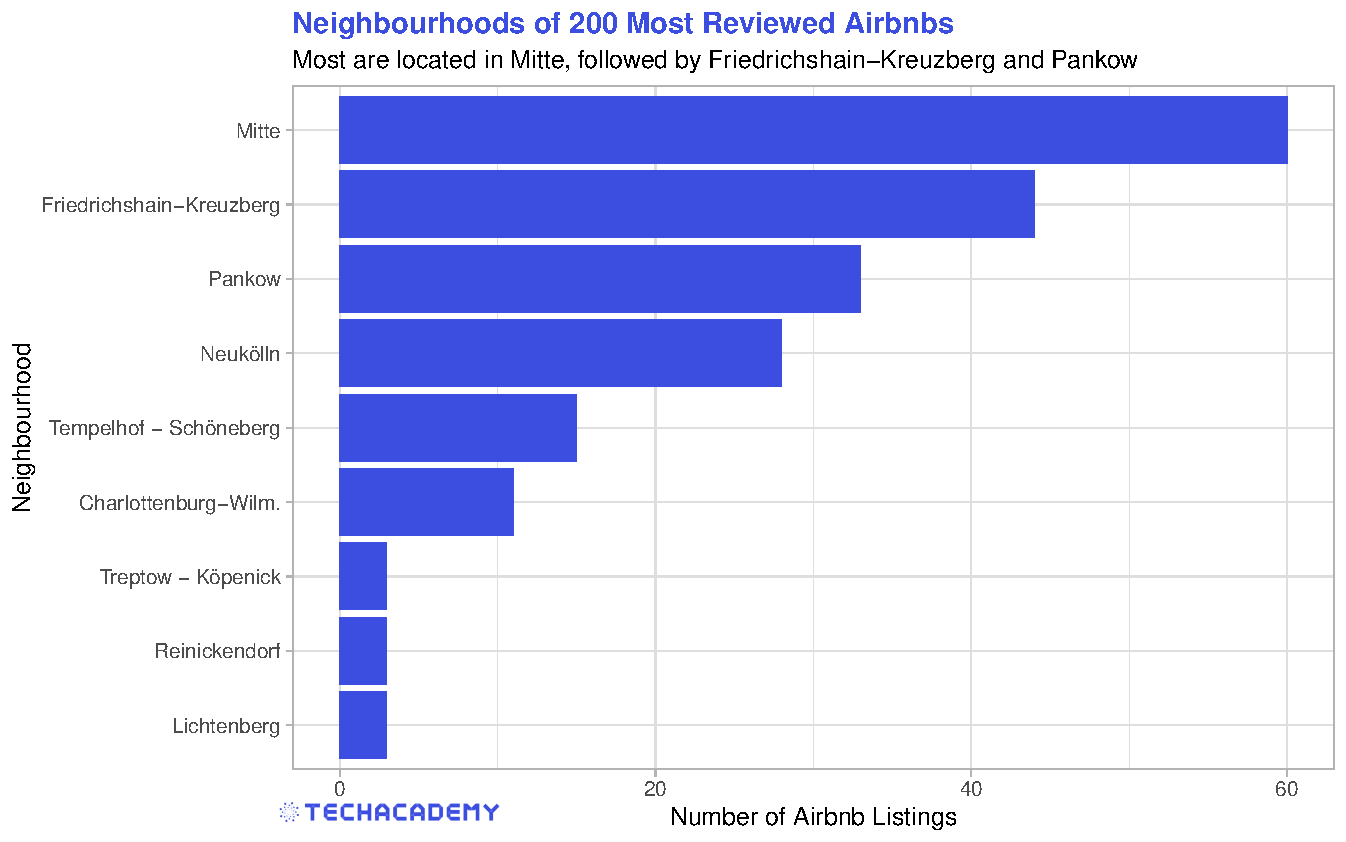
\includegraphics[width=1\linewidth]{plots/3_3_Barplot_MostReviewed}

\hypertarget{geo-daten-mit-karten-visualisieren-listings_reviews}{%
\section{Geo-Daten mit Karten visualisieren (listings\_reviews)}\label{geo-daten-mit-karten-visualisieren-listings_reviews}}

Wer die Internetseite von Airbnb kennt, hat bestimmt auch die Funktion gesehen, die Apartments auf einer Karte anzeigen zu lassen.
Das gleiche können wir auch!
Mit dem Unterschied, dass unsere Daten uns noch mehr Möglichkeiten geben anzuzeigen, was uns wirklich interessiert!

Wie kommen wir praktisch zu unserer Karte?
Es gibt einige unterschiedliche packages, die Karten in R zeichnen können.
Die folgenden Tipps beziehen sich auf \texttt{ggmap}.

Bevor du über eine API-Schnittstelle Kartenmaterial downloaden kannst, musst du die Ecken der Karte als Koordinaten definieren.
Nutze zur Komplexitätsredukion den in der dritten Aufgabe gefilteren kleineren Datensatz mit den 200 am häufigsten rezensierten Apartments für diese Aufgabe.

Definiere zuerst die Höhe und Breite der enthaltenen Koordinaten.

Damit kannst du im nächsten Schritt die genauen Ecken relativ zu den Koordinaten im Datensatz festlegen.
Dies erledigst du in einem Vektor, den du zum Beispiel \texttt{berlin\_borders} nennen kannst.
In diesem sind jeweils Werte für die Kanten der Karte definiert.
Zu den jeweiligen Minima, bzw. Maxima der Koordinaten kannst du noch einen kleinen Sicherheitsabstand hinzufügen.
Spiele später etwas mit den Faktoren herum, um einen guten Kartenausschnitt zu finden.

Danach downloaden wir den definierten Kartenausschnitt vom Dienstleister Stamen Maps mit der Funktion \texttt{get\_stamenmap()} und speichern diesen in einem Objekt.

Jetzt können wir anfangen, Objekte auf der Karte zu platzieren.
Damit die Karte nicht unübersichtlich wird, sollten nicht zu viele Apartments angezeigt werden.
Praktisch ist dafür, dass wir in der letzten Aufgabe bereits eine Vorauswahl (Top 200) getroffen haben, die wir jetzt weiter benutzen können.

Plotte die 200 meistbewerteten Listings (aus Aufgabe 3) auf der Karte!
Wenn du Aufgabe 3 noch nicht gelöst hast, wähle einfach 200 Listings nach anderen Kriterien oder zufällig aus, um die Aufgabe zu lösen.
Das sollte dann in etwa folgendermaßen aussehen:

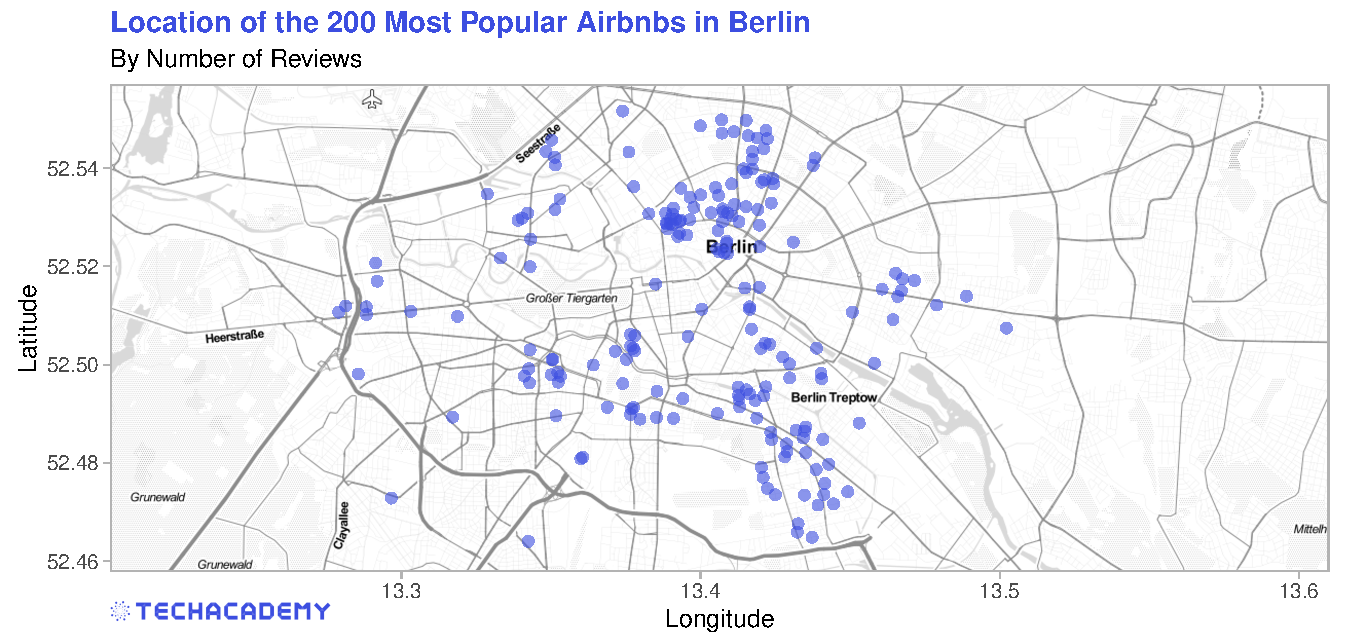
\includegraphics[width=1\linewidth]{plots/4_1_map_top200_simple}

In unseren Daten gibt es über die GPS-Koordinaten hinaus noch viele Informationen zu jedem Listing.
Plotte die Apartments diesmal in unterschiedlichen Farben.
Nutze als Unterscheidungsmerkmal hierfür die Stadtteile (auch um leicht zu sehen, ob die Zuordnung funktioniert).
Unter diesem Absatz findest du ein Beispiel, wie ein etwas fortgeschrittener Plot dazu aussehen kann.
Dieser Plot wurde mit \texttt{ggmaps} und dem zusätzlichen Package \texttt{concaveman} sowie dessen Funktion \texttt{geom\_mark\_hull()} erstellt, welches Polygone um ein Cluster von Koordinaten zeichnet.
Es ist aber ausreichend, wenn du den gleichen Plot wie zuvor, nur mit unterschiedlichen Farben umsetzt.

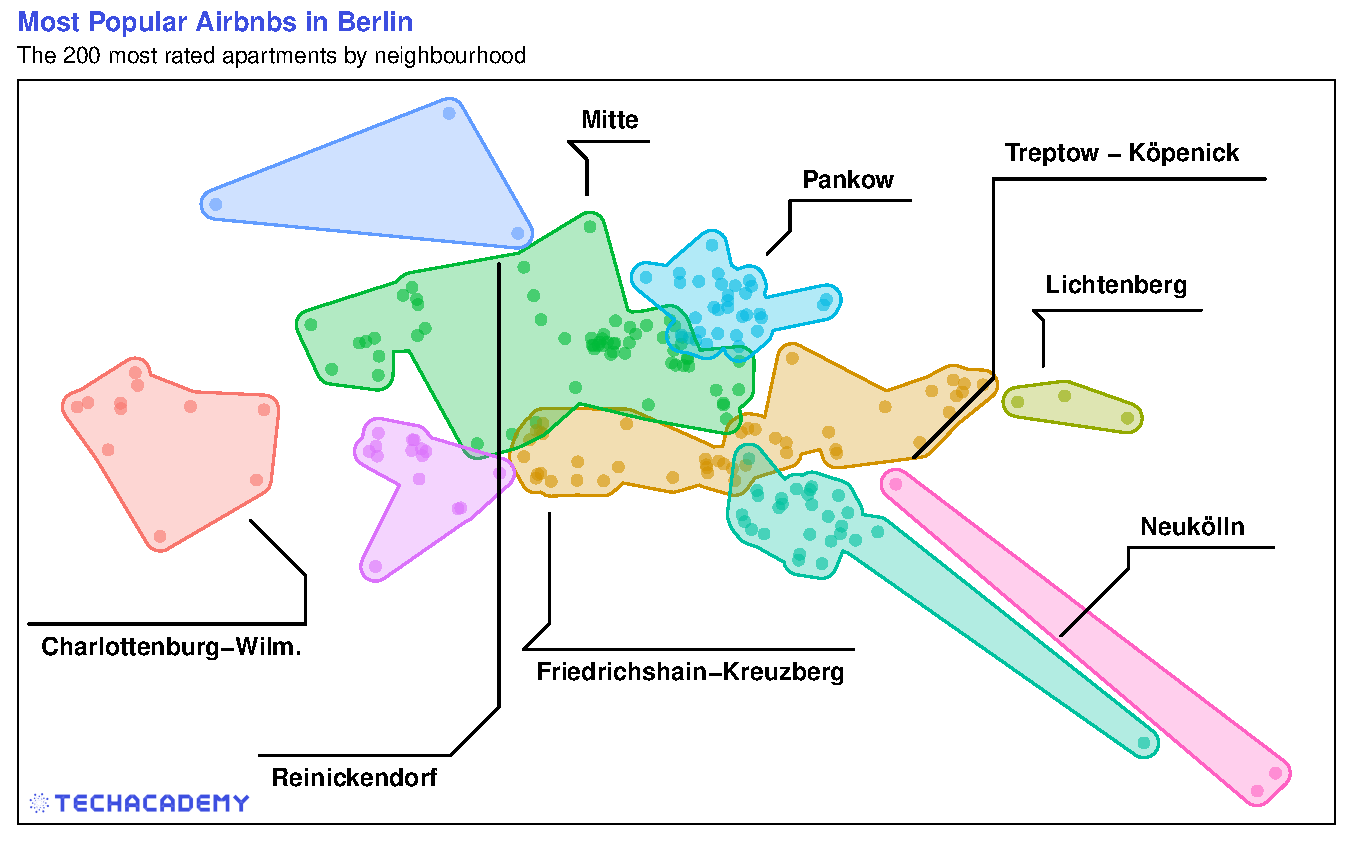
\includegraphics[width=1\linewidth]{plots/4_2_map_top200_by_neighbourhood}

Für einige Analysen ist es leichter, wenn man nicht einfach nur Punkte, sondern dessen Verteilungen auf einer Karte sieht.
Um zum Beispiel zu erkennen, wo sich viele Apartments auf wenig Raum befinden, kannst du dir die Apartment-Dichte anzeigen lassen.
Erstelle einen solchen zweidimensionalen Dichteplot mit \texttt{geom\_density2d()} sowie \texttt{stat\_density2d()}auf der Karte!
Falls du nicht genau weißt, wie die einzelnen Argumente befüllt werden sollen, google dich zu einer Lösung.

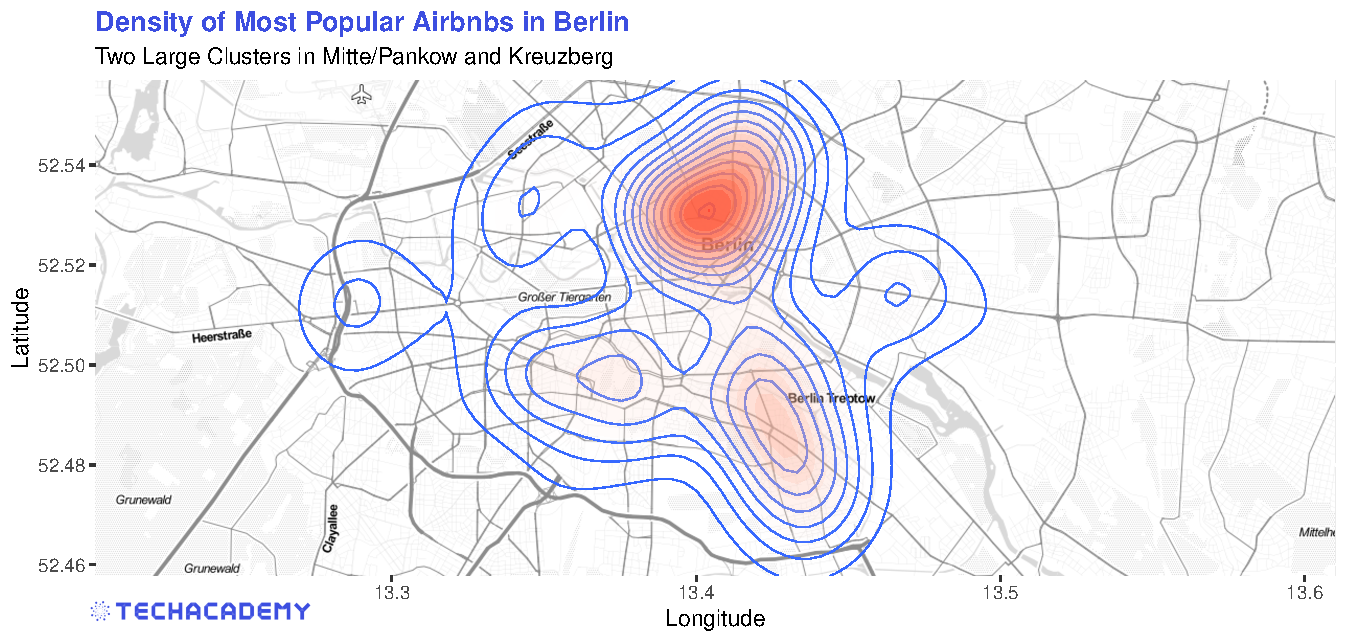
\includegraphics[width=1\linewidth]{plots/4_3_map_top200_density}

Herzlichen Glückwunsch -- Du hast jetzt dank viel Arbeit mit grundlegenden Daten-Transformationen und vieler Visualisierungen ein gutes Grundverständnis des Airbnb-Angebots in Berlin.
Damit hast du den ersten Teil des Projektes erfolgreich abgeschlossen!
Wenn du in der Anfänger-Gruppe bist, sind deine Mindestvoraussetzungen hiermit erfüllt.
Wir empfehlen dir aber trotzdem dringend, dich auch mit dem folgenden Teil auseinanderzusetzen. Denn wir entwickeln jetzt Methoden, um die Zukunft vorauszusagen!
Klingt spannend, oder?

\hypertarget{preisvorhersage-wende-statistische-methoden-an-1}{%
\chapter{Preisvorhersage -- Wende statistische Methoden an}\label{preisvorhersage-wende-statistische-methoden-an-1}}

Im vorherigen Teil hast du ein Gefühl für den Datensatz bekommen. Du weißt jetzt, welche Variablen enthalten sind und kennst ein paar charakteristische Eigenschaften des Datensatzes. Noch haben wir den Datensatz aber nur visualisiert. In diesem Abschnitt gehen wir einen Schritt weiter und wenden statistische Methoden an, um den Preis von einzelnen Airbnb Apartments möglichst genau vorherzusagen.

Um dein Modell am Schluss vergleichen zu können, verwenden wir eine einheitliche Metrik, nach der wir die Preisvorhersagen auf Genauigkeit überprüfen können.
In unserem Fall ist dies der Root Mean Squared Error (\(RMSE\)), also die Wurzel der durchschnittlich quadrierten Differenz zwischen dem vorhergesagten (\(\hat{y}_i\)) und tatsächlichen Wert (\(y_i\)):

\begin{center}
$RMSE = \sqrt{\frac{1}{N}\sum_{i=1}^{N}{(\hat{y}_i-y_i)^2}}$
\end{center}

Je näher der \(RMSE\) an 0 ist, desto besser sagt dein Modell die Preise vorher.
Dein Ziel ist es im Folgenden also den \(RMSE\) deiner verschiedenen Modelle durch kontinuierliche Verbesserungen möglichst weit zu reduzieren.

Wir nutzen für den folgenden Teil drei verschiedene Datensätze, welche du im Unterordner \emph{Full Data Set} findest.
Diese basieren auf einem deutlich umfangreicheren Datensatz, der insgesamt 96 Variablen für jedes Apartment enthält.
Wir haben bereits den Test/Train/Validation split der Daten vorgenommen, damit jede Gruppe mit der gleichen Aufteilung arbeitet.
Hier eine kurze Beschreibung, wofür du die Datensätze benötigst:

\begin{itemize}
\tightlist
\item
  \textbf{train.csv} (60 \%): Diesen Trainings-Datensatz verwendest du, um dein Modell zu trainieren. Das Modell lernt also die Zusammenhänge zwischen den Variablen dadurch kennen.
\item
  \textbf{test.csv} (30 \%): Mit diesem Test-Datensatz kannst du testen, wie gut dein Modell den Preis mit Hilfe von bisher nicht gesehenen Daten vorhersagt. Dabei erkennst du zum Beispiel under-/overfitting.
\item
  \textbf{val.csv} (10 \%): In diesem Validation-Datensatz haben wir die Variable \texttt{price} entfernt. Du wendest am Schluss dein bestes Modell darauf an und schickst uns deine Vorhersagen für \texttt{price}. Wir vergleichen diese dann mit den tatsächlichen (nur uns bekannten) Werten mit Hilfe des \(RMSE\) und küren nach Projektabgabe das beste Modell über alle Gruppen hinweg.
\end{itemize}

Beachte, dass in diesen drei Datensätzen wieder einige Bereinigungen notwendig sind.
So sind zum Beispiel alle Preis-Variablen mit einem \$-Zeichen versehen.
Wir müssen diese entfernen, damit R die Variablen als numerisch interpretieren kann und wir diese für die folgenden Modelle verwenden können. Behalte immer im Hinterkopf, dass du alle Transformationen auf alle drei Datensätze anwenden musst, da du sonst dein trainiertes Modell nicht auf den Test- sowie Validierungsdatensatz anwenden kannst.

\hypertarget{untersuche-die-korrelation-zwischen-den-variablen-nuxe4her-train}{%
\section{Untersuche die Korrelation zwischen den Variablen näher (train)}\label{untersuche-die-korrelation-zwischen-den-variablen-nuxe4her-train}}

Lade zuerst den \texttt{train.csv} Datensatz aus dem Ordner \emph{Full Data Set} in deinen Workspace.
Schaue dir jetzt die Variablennamen und die ersten Einträge an um zu entscheiden, welche Daten für die Vorhersage des Preises nützlich sein können.
Wähle diese (beschränke dich zuerst auf nicht mehr als 20 Variablen) plus \texttt{price} aus und speichere diese in einem neuen data.frame.

Wie stehen einzelne Variablen miteinander in Verbindung?
Sprich inwiefern korrelieren die Variablen des Datensatzes miteinander?
Das herauszufinden ist enorm wichtig für die Entscheidung, welches Modell du später anwenden kannst.\\
Ein guter Anfang ist es, eine Korrelationsmatrix zu erstellen.
Ein Teil dafür ist die Funktion \texttt{cor()} aus dem \texttt{base} package.
Selektiere alle numerische Variablen in deinem Datensatzes mit Hilfe von \texttt{sapply()} und erstelle eine Korrelationsmatrix.

Einen sehr praktischen Plot zur Visualisierung von Zusammenhängen zwischen vielen Variablen liefert das Package \texttt{GGally} mit der Funktion \texttt{ggpairs()}.
Wähle die vier Variablen (und \texttt{price}) aus, die deiner Meinung nach am meisten den Preis beeinflussen und erstelle einen ggpairs-Plot.
Beachte hierbei, dass der Plot schnell unlesbar wird und lange zum Erstellen braucht, sobald du deutlich mehr als fünf Variablen plottest.

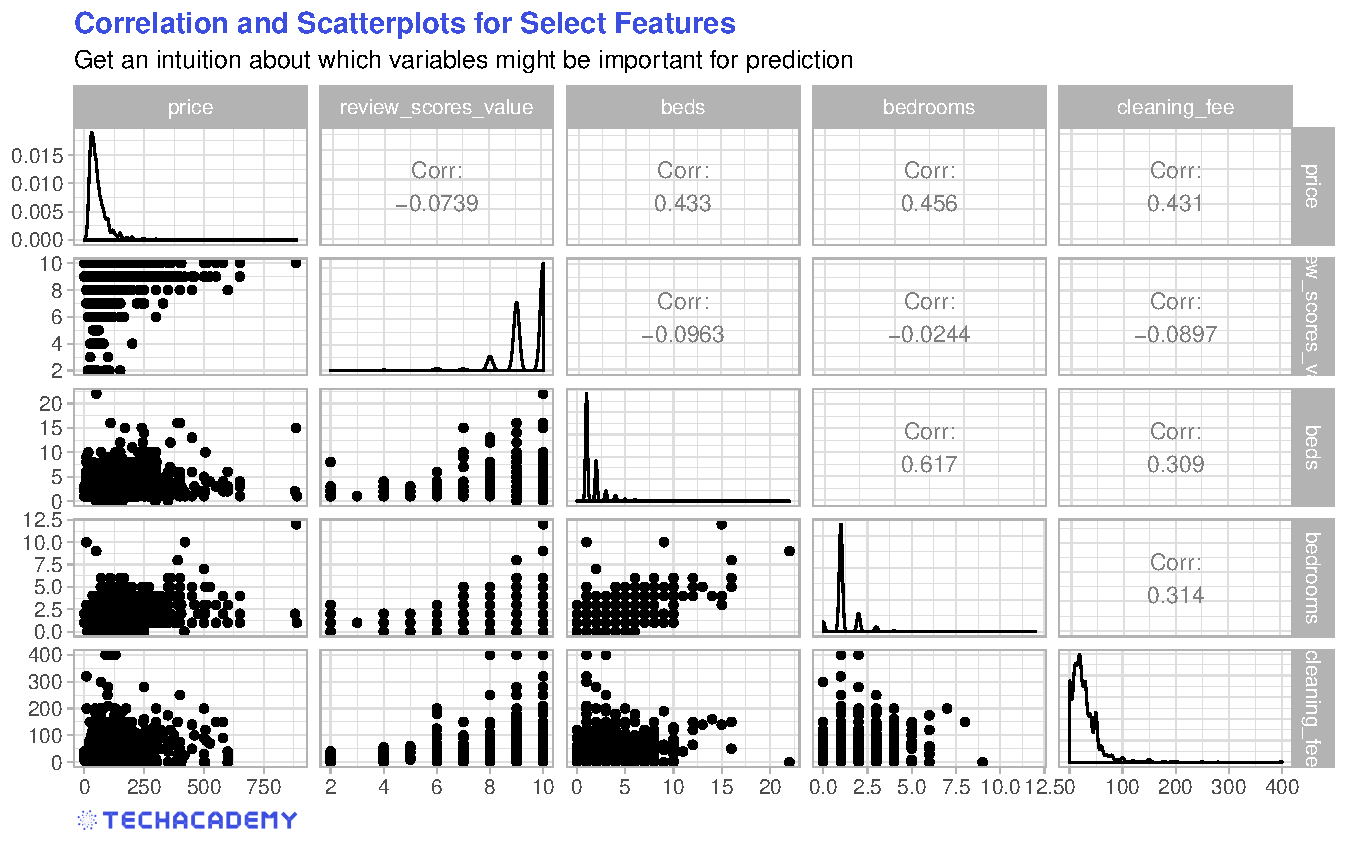
\includegraphics[width=1\linewidth]{plots/5_1_ggpairs}

Welche deiner untersuchten Variablen korreliert am meisten mit dem Preis und welche scheinen eher unabhängig vom Preis zu sein?
Du hast jetzt einen ersten Eindruck, welche Variablen für dein Modell wichtig werden könnnten.
Kommen wir also zu deinem ersten Preis-Vorhersage-Modell!

\hypertarget{erste-vorhersagen-mit-einfachen-regressionsmodellen-train}{%
\section{Erste Vorhersagen mit einfachen Regressionsmodellen (train)}\label{erste-vorhersagen-mit-einfachen-regressionsmodellen-train}}

Jetzt kannst du dich mit deinen Statistik-Kenntnissen austoben:
Du benötigst jetzt ein Verfahren, wie du den Preis eines Airbnb Apartments an einem bestimmten Tag vorhersagen kannst.\\
Eine erste sehr einfache Herangehensweise wäre den Durchschnitt der Nachfrage als erste Vorhersage zu verwenden. Ziemlich sicher ist das jedoch nicht die beste Vorhersage.
Deine vorhergesagter Preis wäre in diesem Fall über alle Tage gleich und würde alle Faktoren, die den Preis beeinflussen, außer Acht lassen.

Schon einmal was von einer linearen Regression gehört? Das wäre ein deutlich besserer Ansatz.
Jetzt kannst du deine Statistik-Skills ausspielen.
Stelle zuerst ein Modell mit der abhängigen Variable \texttt{price} auf.
In der vorherigen Aufgabe hast du unterschiedliche Variablen untersucht.
Suche dir jetzt diejenige Variable mit der höchsten Korrelation zum Preis aus und verwende diese als einzige unabhängige Variable.

Dein erstes Regressionsmodell könnte zum Beispiel so aussehen:

\begin{center} $price = \beta_0 + \beta_1 bedrooms + \epsilon$ \end{center}

In R kannst du eine einfache lineare Regression mit der Funktion \(lm()\) implementieren. Die Ergebnisse davon gibst du dann mit der \(summary()\) Funktion aus.

Hat deine unabhängige Variable einen statistisch signifikanten Einfluss auf den Apartment-Preis?
Vermutlich ja, denn wir haben als einzige die am höchsten zum Preis korrelierte Variable ausgewählt.
Wenn wir jedoch bei diesem sehr vereinfachten Modell bleiben, begehen wir einen typischen Fehler:
Den sogenannten Omitted Variable Bias (OVB).
Grob vereinfacht gesprochen vernachlässigen wir (im Statistik-Jargon: kontrollieren nicht für) Variablen, die einen signifikanten Einfluss auf die abhängige Variable haben.
Man könnte vermuten, dass andere Einflussfaktoren auch eine große Rolle bei der Preisbiildung haben.
Wenn wir diese also nicht mit aufnehmen, ist die Schätzung des Effektes von \(bedrooms\) verzerrt und damit schlecht zu gebrauchen.
In diesem Fall ist das vorerst kein großes Problem für uns, da wir nicht an kausalen Effekten, sondern aussließlich an einer möglichst guten Vorhersage interessiert sind.
Deinem Statistik-Prof würden bei so einem Modell ziemlich sicher die Haare zu Berge stehen.
Nichtsdestotrotz wird dieses Modell mit nur einer einzigen erklärenden Variable den Preis nicht unbedingt gut vorhersagen.

Eine Lösungsmöglichkeit ist, die vernachlässigten Variablen einfach mit in das Modell aufzunehmen --- wie praktisch, dass diese auch schon in dem Datensatz enthalten sind. Stellen wir also ein etwas umfangreicheres Modell auf, das die noch eine weitere Variable mit aufnimmt:

\begin{center} $price = \beta_0 + \beta_1 bedrooms + \beta_2 cleaning\_fee + \epsilon$ \end{center}

Vergleiche nun die Ergebnisse der beiden Modelle.
Erklärt das umfangreichere Modell einen höheren Anteil der Varianz im Preis?
Sprich welches Modell weist dem höheren Wert für das Bestimmtheitsmaß \(R^2\) aus?
Tipp: Solche LaTeX-Tabellen kannst du einfach mit dem \texttt{stargazer} Package in dein RMarkdown Dokument mit aufnehmen.

\begin{table}[!htbp] \centering 
  \caption{Model Summary for Two Simple Linear Regression Models} 
  \label{} 
\begin{tabular}{@{\extracolsep{5pt}}lcc} 
\\[-1.8ex]\hline 
\hline \\[-1.8ex] 
 & \multicolumn{2}{c}{\textit{Dependent variable:}} \\ 
\cline{2-3} 
\\[-1.8ex] & \multicolumn{2}{c}{price} \\ 
\\[-1.8ex] & (1) & (2)\\ 
\hline \\[-1.8ex] 
 bedrooms & 35.317$^{***}$ & 28.715$^{***}$ \\ 
  & (0.594) & (0.642) \\ 
  & & \\ 
 cleaning\_fee &  & 0.576$^{***}$ \\ 
  &  & (0.017) \\ 
  & & \\ 
 Constant & 18.272$^{***}$ & 13.313$^{***}$ \\ 
  & (0.790) & (0.864) \\ 
  & & \\ 
\hline \\[-1.8ex] 
Observations & 13,488 & 9,245 \\ 
R$^{2}$ & 0.208 & 0.331 \\ 
Adjusted R$^{2}$ & 0.208 & 0.331 \\ 
Residual Std. Error & 45.115 (df = 13486) & 39.777 (df = 9242) \\ 
F Statistic & 3,538.208$^{***}$ (df = 1; 13486) & 2,283.658$^{***}$ (df = 2; 9242) \\ 
\hline 
\hline \\[-1.8ex] 
\textit{Note:}  & \multicolumn{2}{r}{$^{*}$p$<$0.1; $^{**}$p$<$0.05; $^{***}$p$<$0.01} \\ 
\end{tabular} 
\end{table}

\hypertarget{von-training-zu-testen-treffe-vorhersagen}{%
\section{Von Training zu Testen -- Treffe Vorhersagen}\label{von-training-zu-testen-treffe-vorhersagen}}

Jetzt hast du dein erstes Modell mit dem Trainings-Datensatz \emph{trainiert}.
Doch wie gut geht das Modell mit Daten um, die es noch nicht gesehen hat?
Das ist ein sehr wichtiger Test um die Qualität deines Modells zu bewerten.

Hat dein Modell nur die vorhandenen Muster im Trainings-Datensatz ``auswendig'' gelernt?
Dann wären die Zusammenhänge aus dem Trainings-Datensatz nicht übertragbar auf den Test-Datensatz.
Beim sogenannten Overfitting hat das Modell zu nah am Trainings-Datensatz gelernt und liefert deshalb schlechte Vorhersagen bei unbekannten Daten --- zum Beispiel in deinem Test- und Validierungs-Datensatz.\\
Auf der andern Seite gibt es auch das Problem Underfitting: Dein Modell hat die tatsächlichen Zusammenhänge der Daten nicht ausreichend gelernt und sagt deshalb in dem Test-Datensatz schlecht voraus.
Es gilt also, die goldene Mitte zwischen den beiden Problemen zu finden.

Jetzt wird die Unterscheidung zwischen Trainings- und Testdatensatz wichtig. Zur Erinnerung: wir nutzen \texttt{train}, um ein Modell zu \textbf{trainieren} und \texttt{test}, um die Qualität unseres Modells letztendlich zu \textbf{testen}.

Lade nun zusätzlich zu dem Datensatz \texttt{train}, den du bereits vorher verwendet hast, den Datensatz \texttt{test}.
Um nun dein Modell an bisher ungesehenen Daten zu testen, kannst du das Modell auf den \texttt{test} Datensatz anwenden.
Nutze dafür die Funktion predict:

Damit hast du einen Vektor mit allen Preisvorhersagen für den \texttt{test} Datensatz erstellt.
Diesen kannst du jetzt mit den tatsächlichen Werten für \texttt{price} aus \texttt{test} vergleichen.
Um eine einheitliche Vergleichsmetrik zu verwenden, nutze bitte folgende Funktion zur Messung deiner Vorhersagegenauigkeit.

Vergleiche nun beide Regressionsmodelle.
Hat das umfangreichere Modell bessere Vorhersagegenauigkeit, also einen niedrigeren \(RMSE\)?
Jetzt hast du einen Benckmark für deine fortgeschritteneren Modelle, den es im nächsten Teil zu schlagen gilt.

\hypertarget{wende-fortgeschrittene-machine-learning-algorithmen-an}{%
\section{Wende fortgeschrittene Machine Learning-Algorithmen an}\label{wende-fortgeschrittene-machine-learning-algorithmen-an}}

Nachdem du jetzt eine erste Vorhersage mit Hilfe eines einfachen Regressionsmodells erstellt und getestet hast, kannst du dich jetzt an fortgeschrittenere Methoden herantasten.
Das Ziel ist immer noch, einen möglichst niedrigen \(RMSE\) beim Anwenden des Modells auf dem \texttt{test} Datensatz zu erhalten.
Suche dir jetzt mindestens einen anderen Algorithmus heraus und überprüfe letztendlich, ob du dadurch eine akkuratere Vorhersage (ausgedrückt durch niedrigeren \(RMSE\)) erhältst.
Inspirationen dazu findest du bei den fortgeschrittenen DataCamp-Kursen, welche am Anfang des Leitfadens aufgelistet sind.
Dir sind dabei keine Grenzen gesetzt -- du kannst die Regression durch bestimmte Verfahren verfeinern (z.B. LASSO) oder gleich ein Random Forest Modell oder ein Neuronales Netzwerk aufstellen.
Es ist meistens eine gute Idee, sich kurz die Funktionsweise der jeweiligen Algorithmen in Erinnerung zu rufen und zu überlegen, ob diese Methodik in diesem Fall bei einer kontinuierlichen Vorhersagevariable Sinn macht.

An dieser Stelle ist ein Hinweis angebracht: Unser Datensatz hat über viele Variablen teilweise einen substantiellen Teil an fehlenden Beobachtungen (\texttt{NA}).
Einige Machine Learning Algorithmen verlangen einen vollständigen Datensatz ohne Missing Values, während andere mit einer kleineren Anzahl gut zurecht kommen.
Überprüfe also zuerst, ob du die Missing Values durch ein bestimmtes Verfahren imputieren\footnote{"imputieren" bedeutet, dass du deine `NA` durch einen Wert ersetzt, der auf Basis der restlichen Werte oder den anderen Variablen berechnet wird. So kannst du zum Beispiel den fehlenden Wert durch eine Regression auf die restlichen Variablen vorhersagen} kannst.
Welche Methode dafür am besten geeignet ist, hängt stark von deinem Vorhersage-Algorithmus ab.

Zudem kannst du einen spürbaren Zugewinn an Vorhersagekraft erhalten, indem du bestehende Variablen modifizierst oder neue Variablen aus dem Datensatz generierst (``feature engineering'').
Zum Beispiel könnten wir uns vorstellen, dass die Distanz eines Apartments zum Stadtzentrum einen deutlichen Einfluss auf den Preis hat.
Diese Variable ist jedoch nicht in unserem Datensatz enthalen.
Du kannst jedoch eine einfache Funktion schreiben, die mit Hilfe der zwei Koordinaten-Variablen die Distanz zum Zentrum Berlins berechnet und diese als neue Variable an den Datensatz anhängt.

Vergleiche immer den \(RMSE\) deiner fortgeschrittenen Modelle unterienander, sowie im Vegleich zu dem Benckmark Regressionsmodell.

Du hast dein bestes Modell gefunden? Dann wende wie oben die Funktion \texttt{predict()} mit deinem Gewinnermodell an -- dieses mal jedoch auf den Validierungs-Datensatz \texttt{val}.

Schicke in Anhang deiner Projektabgabe einen .csv Datensatz in folgendem Format mit den beiden einzigen Variablen \texttt{id} und \texttt{predicted\_price} mit.

\begin{table}[!htbp] \centering 
  \caption{Submission Format} 
  \label{} 
\begin{tabular}{@{\extracolsep{5pt}} ccc} 
\\[-1.8ex]\hline 
\hline \\[-1.8ex] 
id & predicted\_price \\ 
\hline \\[-1.8ex] 
2015 & $113$ \\ 
2695 & $9$ \\ 
3176 & $137$ \\ 
\vdots & \vdots \\
28089647 & $25$ \\ 
5012107 & $78$ \\ 
\hline \\[-1.8ex] 
\end{tabular} 
\end{table}

Dies erreichst du, indem du die beiden Vektoren \texttt{id} und \texttt{predicted\_price} aneinanderfügst und als .csv Datei abspeicherst.

Damit hast du alle Aufgaben bearbeitet!
Wir hoffen du hattest Spaß beim Programmieren und hast einige spannende Methoden in R gelernt.
Vergesse nicht, dein PDF Dokument und die eben generierte .csv Datei vor der Deadline an unsere Projektabgabe-Email-Adresse zu schicken.

\hypertarget{noch-fragen}{%
\chapter{Noch Fragen?}\label{noch-fragen}}

Du kommst nicht weiter? Willst dein Modell noch weiter verbessern, weißt aber nicht genau wie? Oder dir fällt gerade nicht ein, wie man etwas bestimmtes im Code umsetzt? Schaue dir noch einmal unser Handbuch an. Dort findest du hilfreiche Hinweise, wie du in diesem Fall weiter verfahren und wo du nach einer Lösung für deine Fragestellung suchen kannst.

\hypertarget{anhang}{%
\chapter{Anhang}\label{anhang}}

\hypertarget{aufgaben-checkliste-fuxfcr-das-airbnb-data-science-projekt}{%
\section{Aufgaben-Checkliste für das Airbnb Data Science Projekt}\label{aufgaben-checkliste-fuxfcr-das-airbnb-data-science-projekt}}

\textbf{Exploratory Data Analysis (Anfänger + Fortgeschrittene)}

\begin{enumerate}
\def\labelenumi{\arabic{enumi}.}
\item
  Visualisieren der verfügbaren Apartments (calendar dataset):

  1.1 Wandle die Werte t/f zu \texttt{true} bzw. \texttt{false} um

  1.2 Aggregiere die Daten nach dem Datum

  1.3 Plotte die Anzahl der verfügbaren Apartments über die Zeit
\item
  Visualisieren des listings Datensatz

  2.1 Bereinige und transformiere die Spalten \texttt{price} und \texttt{cleaning\_fee} zu \texttt{numeric}-Werten

  2.2 Bestimme mean und standard deviation des Apartment-Preises nach Stadtteil

  2.3 Visualisiere die Preisverteilung des teuersten und günstigsten Stadtteils

  2.4 Visualisiere, ob die \texttt{cleaning\_fee} benutzt wird um die Preise versteckt zu erhöhen
\item
  Merging des \texttt{listings} und \texttt{review} Datensatzes

  3.1 Aggregiere die Reviews anhand der \texttt{ID}

  3.2 Merge \texttt{listings} und den aggregierten Reviews Datensatz

  3.3 Filtere Apartments und plotte die Anzahl dieser in einem Barplot nach Stadtteil
\item
  Visualisiere die Apartments auf einer Karte

  4.1 Zeiche einen Punkt für jedes zur Verfügung stehende Apartment auf eine Karte

  4.2 Färbe die Punkte unterschiedlich, je nachdem in welchem Stadteil sie sind

  4.3 Erstelle eine 2d-Density Plot der Apartments auf einer Karte
\end{enumerate}

\textbf{Preisvorhersage mit statistischen Verfahren (Fortgeschrittene und ambitionierte Anfänger)}

\begin{enumerate}
\def\labelenumi{\arabic{enumi}.}
\item
  Visualisiere die Korrelationen der Features mit einer Heatmap
\item
  Regression

  2.1 Einfaches Regressionsmodel mit einer erklärenden Variable

  2.2 Regressionsmodel mit zwei oder mehr Features
\item
  Testen der Modelle

  3.1 Benutze den Testdatensatz um Preise für die Apartments vorherzusagen

  3.2 Vergleiche deine Prognosen mit den tatsächlichen Preisen mit Hilfe des RMSE

  3.3 Implementiere einen fortgeschrittenen Algorithmus und sende uns dein bestes Ergebnis zu
\end{enumerate}

\hypertarget{beschreibung-der-variablen-in-den-datensuxe4tzen}{%
\section{Beschreibung der Variablen in den Datensätzen}\label{beschreibung-der-variablen-in-den-datensuxe4tzen}}

\begin{tabular}{ll}
\toprule
                        \textbf{Name} &                 \textbf{Beschreibung} \\
\midrule
                           id &                        Identifikationsnummer \\
                        price &                                        Preis \\
 neighbourhood\_group\_cleansed &                                 Stadtviertel \\
                     latitude &                                  Breitengrad \\
                    longitude &                                   Längengrad \\
                    bathrooms &                        Anzahl an Badezimmern \\
              availability\_30 &       Verfügbarkeit in den nächsten 30 Tagen (Tage) \\
             availability\_365 &               Verfügbarkeit im nächsten Jahr (Tage) \\
                         beds &                             Anzahl an Betten \\
                     bedrooms &                          Anzahl Schlafzimmer \\
          review\_scores\_value &                          Bewertungspunktzahl \\
                     bed\_type &                        Beschreibung zum Bett \\
               minimum\_nights &            minimale Anzahl an Übernachtungen \\
               maximum\_nights &            maximale Anzahl an Übernachtungen \\
                property\_type &  Art des Angebotes: (Appartment, Zimmer,...) \\
     is\_business\_travel\_ready &                für Geschäftsreisen geeignet? \\
                 cleaning\_fee &                              Reinigunsgebühr \\
                    room\_type &                              Art des Zimmers \\
                  square\_feet &                         Größe in square feet \\
              guests\_included &             Sind Gäste im Preis inbegriffen? \\
\bottomrule
\end{tabular}

  \bibliography{book.bib,packages.bib}

\end{document}
